\documentclass[11pt,a4paper]{article}
\usepackage[T1]{fontenc}
\usepackage[utf8]{inputenc}
\usepackage{lmodern}
\usepackage[a4paper, margin=2.5cm]{geometry}
\usepackage{graphicx}
\usepackage{longtable}
\usepackage{booktabs}
\usepackage{float}
\usepackage{listings}
\usepackage{xcolor}
\usepackage{hyperref}
\usepackage{parskip}
\usepackage{microtype}
\usepackage{titlesec}

\hypersetup{
    colorlinks=true,
    linkcolor=blue!60!black,
    urlcolor=blue!60!black,
}

\lstset{
    basicstyle=\ttfamily\small,
    breaklines=true,
    backgroundcolor=\color{gray!10},
    frame=single,
    framesep=4pt,
    xleftmargin=4pt,
    xrightmargin=4pt,
}

\titleformat{\section}{\large\bfseries}{}{0em}{\thesection\quad}
\titleformat{\subsection}{\normalsize\bfseries}{}{0em}{\thesubsection\quad}
\titlespacing{\section}{0pt}{16pt}{6pt}
\titlespacing{\subsection}{0pt}{10pt}{4pt}

\begin{document}

\section{Log-to-Vec Benchmark --- Comprehensive Research Report}

\textit{Generated: 2026-05-07}

\vspace{4pt}\hrule\vspace{4pt}

\subsection{1. Project Goal}

Learn useful \textbf{embeddings of PLC/SCADA log files} for mode-change detection and regime
identification in industrial control systems. The logs are timestamped records of sensor readings
and discrete machine state codes --- essentially serialised multivariate time series with no
meaningful free text.

The motivating question: can a learned representation capture operating regime, load, and
mode-change structure \textbf{without hand-labelled data}, well enough to be useful downstream?

\vspace{4pt}\hrule\vspace{4pt}

\subsection{2. Session Log}

Each row records one working session: what we set out to do, what ran on Alvis, and what the
session established. Dates are commit dates (UTC+1). All cluster jobs ran on Alvis (Chalmers
HPC) using A40/A100 GPUs unless noted.

\begin{longtable}{|l|l|l|l|l|}
\hline
\textbf{Date} & \textbf{Session} & \textbf{Aim} & \textbf{Key actions} & \textbf{Outcome / what we learned} \\
\hline
\endfirsthead
\hline
\textbf{Date} & \textbf{Session} & \textbf{Aim} & \textbf{Key actions} & \textbf{Outcome / what we learned} \\
\hline
\endhead
\hline
\endfoot
2026-02-06 & S0 --- Repo init & Establish a shared codebase for the log-to-vec study after two failed prototype phases & Initial commit: project layout, shared utilities, history notes & Baseline for all future experiments \\
\hline
2026-04-28 & S1 --- Unify & Merge several prototype branches (LSTM contrastive, TCN hybrid, FRS benchmark) into one coherent repo & Integrated branch code paths, experiment scaffolding, merge ledger & Single working repo; Phase 1--2 retrospective documented; decision to pivot to pretrained foundation model evaluation \\
\hline
2026-04-29 & S2 --- Alvis deploy + RQ2 scaffold & Get the full pipeline running on Alvis GPU cluster; design and submit the first geometry-metric experiment (RQ2) & Apptainer container deployed on Alvis; RQ2 trace comparison scaffolded (3 synthetic problems: P1 simple, P2 multichannel, P3 hard/noisy); SLURM job submitted; retrospective and roadmap written & Container confirmed working; RQ2 job submitted successfully; roadmap committed \\
\hline
2026-04-30 & S3 --- RQ2 fix & MOMENT embedding step crashed: model requires exactly 512-sample input but windows were 128 samples & Pad all windows to 512 before MOMENT forward pass (zero-padding, right-sided); add missing \texttt{\#SBATCH --gpus-per-node} SLURM directive & RQ2 resubmitted and completed; MOMENT padding approach confirmed as viable \\
\hline
2026-05-05 & S4 --- Metric upgrade + RQ4/RQ5 & Add silhouette score and UMAP visualisation to the eval suite; design and run more realistic experiments & Added silhouette score to all geometry metrics; added UMAP plots; scaffolded and submitted RQ4 (CNC-analogous 10-channel benchmark with 7 scenarios and 2 label levels) and RQ5 (window-size sweep ws∈\{32,64,128,256,512\}); fixed sklearn 1.5+ API break in silhouette call; fixed DCC module import error & RQ4 and RQ5 both completed on cluster; silhouette provides cleaner separability signal than MSI alone; sklearn 1.5 compat issue resolved \\
\hline
2026-05-05 & S4b --- SLURM master & Submit all remaining pipeline stages as single GPU jobs with a master submit script & Full-pipeline SLURM jobs (embed$\rightarrow$metrics$\rightarrow$report) added for all RQs; master \texttt{submit\_all.sh} script added & All RQs queued in one command \\
\hline
2026-05-06 & S5 --- RQ3 results + report & Pull RQ3 landscape sweep results (14 scenarios × 5 models) and write first comprehensive report & RQ3 results collected; cross-experiment synthesis written; \texttt{comprehensive\_report.md} v1 written and PDF generated via \texttt{build\_pdf.py} & First full report covering RQ1--RQ5; identified MOMENT/FFT role reversal; documented signal-type failure mode \\
\hline
2026-05-07 & S6 --- RQ6 results + permissions & Collect RQ6 signal-ablation results; update report with session log and full RQ6 section; tidy project permissions & Cluster check: no jobs running; RQ6 results present (24 rows: ratio\_0step$\rightarrow$ratio\_4step + chirp/damped/sawtooth); permissions consolidated in settings.local.json; this report generated & RQ6 confirms MOMENT degrades gracefully with step-channel contamination; exotic signal types (chirp, damped, sawtooth) favour MOMENT strongly \\
\hline
\end{longtable}

\vspace{4pt}\hrule\vspace{4pt}

\subsection{3. Phase 1 --- Contrastive LSTM on Toy Logs}

\textbf{Setup}
\begin{itemize}
  \item LSTM encoder trained with NT-Xent contrastive loss.
  \item Positive pairs: temporal neighbours within a trajectory.
  \item Data: toy CSV logs generated synthetically; sine-wave generator examples.
  \item Evaluation: ad-hoc clustering and retrieval visualisations only. No formal metric suite.
\end{itemize}

\textbf{Outcome}
No quantitative results recorded. Discontinued because:
\begin{enumerate}
  \item Temporal-neighbour positives teach "what is nearby in time", not "what shares a mode".
  \item Toy logs had no ground-truth factorised labels --- claims about quality were unverifiable.
\end{enumerate}

\textbf{Lesson:} A controlled synthetic benchmark with known latent structure is a prerequisite before
any learning claim can be made.

\vspace{4pt}\hrule\vspace{4pt}

\subsection{4. Phase 2 --- TCN Hybrid on FSSS (version2 branch)}

\textbf{Setup}
\begin{itemize}
  \item TCN (Temporal Convolutional Network) with dilated residual conv blocks.
  \item Hybrid loss: NT-Xent contrastive + reconstruction (masked span, Gaussian noise, time shift).
  \item Data: FSSS datasets --- earlier, smaller synthetic variants of FRS.
  \item Formal eval suite added: linear and RBF probes, retrieval@K, clustering ARI.
  \item Baselines: raw statistics, FFT, PCA.
\end{itemize}

\textbf{Results (RBF probe balanced accuracy)}

\begin{longtable}{|l|l|l|l|}
\hline
\textbf{Factor} & \textbf{Baseline (best)} & \textbf{Learned (best)} & \textbf{Delta} \\
\hline
\endfirsthead
\hline
\textbf{Factor} & \textbf{Baseline (best)} & \textbf{Learned (best)} & \textbf{Delta} \\
\hline
\endhead
\hline
\endfoot
mode\_id & 0.277 & 0.267 & $-$0.010 --- \textbf{baseline wins} \\
\hline
spectral\_id & 0.701 & 0.653 & $-$0.048 --- \textbf{baseline wins} \\
\hline
coupling\_id & 0.413 & 0.423 & +0.010 --- marginal \\
\hline
transition & 0.558 & 0.534 & $-$0.024 --- \textbf{baseline wins} \\
\hline
mean\_load & $\approx$0 & $\approx$0 & tied at zero \\
\hline
\end{longtable}

Retrieval R@5 was misleadingly high (0.961--0.993) due to temporal-neighbour training bias.
Clustering ARI was very poor (0.020--0.134).

\textbf{Lesson:} TCN + temporal-neighbour contrastive + reconstruction does not extract factorised
structure. The objective is misaligned with the evaluation goal. Baselines are formidable.

\vspace{4pt}\hrule\vspace{4pt}

\subsection{5. Problem Setups and Datasets}

This section describes all five experimental setups in detail. Each was designed to probe a
specific question about embedding quality, building from simple factor recovery (RQ1) to
realistic multi-channel industrial signals (RQ4/RQ5).

\subsubsection{5.1 RQ1 --- FRS: Factorised Regime Sequence Benchmark}

\textbf{Motivation.} After Phase 1--2 failures, we needed a synthetic benchmark with \textit{known}, \textit{independent}
latent factors and a trajectory-level data split. The FRS generator was purpose-built for this.

\textbf{Data generation.} Each trajectory is a multivariate time series drawn from a hidden Markov model
over a product space of four independent factors:

\begin{itemize}
  \item \textbf{Mode ID} --- discrete operating regime (0--7). Each mode assigns a characteristic sine-wave
\end{itemize}
  frequency and phase to each channel. Modes are randomly ordered within a trajectory and recur.
\begin{itemize}
  \item \textbf{Spectral ID} --- global frequency scaling (3 levels). All channels share the same spectral class
\end{itemize}
  within a trajectory; different trajectories may differ. This tests whether the embedding captures
  a slow-changing global property.
\begin{itemize}
  \item \textbf{Coupling ID} --- cross-channel interaction strength (3 levels: 0 = independent, 1 = moderate,
\end{itemize}
  2 = strong). Coupling is implemented as a weighted additive mixture across channels.
\begin{itemize}
  \item \textbf{Load} --- continuous amplitude multiplier (uniform on [0.5, 2.0]). Represents the overall
\end{itemize}
  signal energy level. Deliberately not separable from mode without amplitude-sensitive learning.

Two datasets are used: \texttt{frs\_clean\_vnext\_long} (additive Gaussian noise $\sigma$ = 0.05) and
\texttt{frs\_noisy\_vnext\_long} ($\sigma$ = 0.20). Each has 200 trajectories of 4000 time steps, 4 channels,
with a \textbf{trajectory-level 70/15/15 train/val/test split} to prevent any leakage of temporal
structure between sets.

\textbf{Why this setup is hard.} The four factors are independent by construction, so the optimal
embedding would factorise along all four axes simultaneously. The load factor is especially hard:
it is a multiplicative scalar on the signal amplitude, and no method we tested recovered it
(R$^2$ $\leq$ 0 throughout). FFT amplitude spectra partially capture amplitude but conflate it with mode
frequency; contrastive learning with temporal neighbours teaches temporal proximity, not amplitude
level.

\textbf{Evaluation suite.} For each factor:
\begin{itemize}
  \item \textbf{RBF SVM probe} --- balanced accuracy on test set (primary metric).
  \item \textbf{Linear SVM probe} --- measures linear separability specifically.
  \item \textbf{Precision@10 retrieval} --- does the nearest neighbour in embedding space share the same factor value?
  \item \textbf{K-Means ARI} --- does unsupervised clustering align with factor labels?
  \item \textbf{Transition detection} --- can mode changes be detected from the embedding sequence?
\end{itemize}

\subsubsection{5.2 RQ2 --- Trace Geometry: Three Synthetic Problems}

\textbf{Motivation.} Probe accuracy tells us about label recovery, but not about the \textit{geometry} of the
embedding space. For online mode-change detection, we care whether the embedding produces
consistent, compact, closed-orbit trajectories --- one orbit per mode --- and whether transitions
between modes are sharp. RQ2 was designed to measure this directly.

\textbf{Problem definitions.} Three problems of increasing difficulty, all modelled on CNC-machining
analogies (each "mode" corresponds to a machining pass):

\begin{itemize}
  \item \textbf{P1 --- Simple 1D.} One channel. Three modes with clearly separated frequencies (0.05, 0.20,
\end{itemize}
  0.40 Hz). Low noise ($\sigma$ = 0.02). This is the easiest possible case: a raw FFT amplitude spectrum
  is expected to trivially separate the modes.
\begin{itemize}
  \item \textbf{P2 --- Multi-channel.} Four channels. Frequencies are similar across channels but combined with
\end{itemize}
  cross-channel mixing (mode 0 emphasises ch0+ch1, mode 1 emphasises ch1+ch2, etc.). Low noise.
  The spectral structure is still clear but requires joint reasoning across channels.
\begin{itemize}
  \item \textbf{P3 --- Hard/Noisy.} Four channels. Frequencies are close across modes (0.10, 0.15, 0.20 Hz).
\end{itemize}
  High noise ($\sigma$ = 0.20). Designed to stress-test all methods --- even FFT struggles when frequency
  separation is small and signal-to-noise is low.

Each problem has 30 trajectories: 15 train, 15 test. Each trajectory visits each mode 5 times
for a total of 15 mode segments. Window size is 128 samples.

\textbf{Geometry metrics.} Five metrics are computed on test-set embeddings:

\begin{longtable}{|l|l|l|l|}
\hline
\textbf{Metric} & \textbf{Symbol} & \textbf{Direction} & \textbf{Meaning} \\
\hline
\endfirsthead
\hline
\textbf{Metric} & \textbf{Symbol} & \textbf{Direction} & \textbf{Meaning} \\
\hline
\endhead
\hline
\endfoot
Mode Separability Index & MSI & $\uparrow$ better & Ratio of inter-mode centroid distance to mean intra-mode spread \\
\hline
Loop Consistency & Loop DTW & $\downarrow$ better & Average DTW distance between repeated visits to the same mode \\
\hline
Transition Sharpness & Trans. Sharp & $\downarrow$ better & Number of windows to cross the embedding midpoint after a mode change \\
\hline
PCA Compactness & PCA Compact & $\downarrow$ better & Convex hull area of the mode trajectory projected to PC1--PC2 \\
\hline
Centroid Stability & Centroid Stab & $\downarrow$ better & Standard deviation of per-run mode centroids across test trajectories \\
\hline
\end{longtable}

\subsubsection{5.3 RQ3 --- Landscape Sweep: 14 Stress Scenarios}

\textbf{Motivation.} RQ1 and RQ2 used one noise level and one signal type. Before recommending any
method for production, we need to know \textit{where} each method's performance degrades. RQ3 sweeps
four independent axes while holding everything else fixed.

\textbf{Base scenario.} 3 modes, 4 channels, sine-wave signal, $\sigma$\_noise = 0.05, no missing data
(identical to the P2 problem in RQ2 but evaluated with the trace-geometry metric suite).

\textbf{Sweep axes and levels:}

\begin{longtable}{|l|l|l|}
\hline
\textbf{Axis} & \textbf{Scenario IDs} & \textbf{Description} \\
\hline
\endfirsthead
\hline
\textbf{Axis} & \textbf{Scenario IDs} & \textbf{Description} \\
\hline
\endhead
\hline
\endfoot
Noise & noise\_000, noise\_020, noise\_040 & $\sigma$ ∈ \{0.00, 0.20, 0.40\} \\
\hline
Missing data & miss\_rand10, miss\_rand30 & Random point dropout, 10\% or 30\% \\
\hline
Missing data & miss\_block30 & Contiguous 30\% block zeroed out \\
\hline
Missing data & miss\_channel & One entire channel zeroed ($\sigma$=0.05) \\
\hline
Number of modes & modes\_2, modes\_5, modes\_8 & K ∈ \{2, 5, 8\} modes \\
\hline
Signal type & sig\_step & Step-change signals (no spectral content) \\
\hline
Signal type & sig\_event & Sparse impulse events \\
\hline
Signal type & sig\_mixed & Mix of sine and step signals \\
\hline
\end{longtable}

\textbf{Why signal type matters.} The two pretrained foundation models we evaluate (MOMENT, and the
FFT baseline which implicitly assumes periodic structure) are both tuned to periodic signals.
Step and event signals expose a fundamental assumption mismatch: neither amplitude spectrum nor
a transformer pretrained on smooth time series handles abrupt non-periodic transitions well.

\textbf{Models evaluated.} FFT8 (8 frequency bins per channel), FFT32 (32 bins per channel), and
MOMENT-1-base. Note: MOMENT was not evaluated on the \texttt{miss\_channel} scenario --- the zero-padded
channel produces degenerate embeddings and was excluded.

\subsubsection{5.4 RQ4 --- CNC-Analogous Mixed-Signal Benchmark}

\textbf{Motivation.} FRS and P1--P3 are purely synthetic sine-wave datasets. Real industrial signals
(PLC/SCADA, CNC machines) have discrete state codes, mixed periodic and aperiodic channels, and
multi-level label structure. RQ4 builds a more realistic benchmark modelled on CNC machining.

\textbf{Signal structure.} 10 channels representing a machining centre:

\begin{longtable}{|l|l|l|l|}
\hline
\textbf{Channel} & \textbf{Unit} & \textbf{Type} & \textbf{Description} \\
\hline
\endfirsthead
\hline
\textbf{Channel} & \textbf{Unit} & \textbf{Type} & \textbf{Description} \\
\hline
\endhead
\hline
\endfoot
axis\_x, axis\_y, axis\_z & mm & continuous & Absolute toolpath position \\
\hline
spindle\_speed & RPM & continuous & Continuous spindle signal \\
\hline
feed\_rate & mm/min & continuous & Commanded feed \\
\hline
vibration\_x, vibration\_y & m/s$^2$ & periodic & Cutting vibration, cutting-freq tied to spindle \\
\hline
temperature & °C & slow continuous & Thermal lag of machining activity \\
\hline
tool\_id & int (0--5) & discrete (float) & Tool currently in spindle \\
\hline
alarm\_code & int (0--99) & discrete (float) & 0 = normal; non-zero = active fault code \\
\hline
\end{longtable}

\textbf{Two-level label structure.} This is the key novelty of RQ4. Every window has \textit{two} ground-truth
labels that represent the same signal at different resolutions:

\begin{itemize}
  \item \textbf{program\_step\_id} --- which G-code block is executing. Fine-grained industrial KPI: can an
\end{itemize}
  embedding distinguish "roughing pass, tool 2" from "finishing pass, tool 3"?
\begin{itemize}
  \item \textbf{op\_state\_id} --- coarse operating state: IDLE (0), HOMING (1), RAPID (2), CUTTING (3),
\end{itemize}
  DWELL (4), FAULT (5). Represents PLC-visible machine state, independent of the specific program.

Both labels are used independently as grouping variables for the metric suite. This lets us ask:
does an embedding that separates operating states also separate program steps, or do the two tasks
require different representations?

\textbf{Seven scenarios.} Each scenario holds the machining program fixed and varies one aspect:

\begin{longtable}{|l|l|l|l|}
\hline
\textbf{Scenario} & \textbf{Programs} & \textbf{Runs} & \textbf{Key variation} \\
\hline
\endfirsthead
\hline
\textbf{Scenario} & \textbf{Programs} & \textbf{Runs} & \textbf{Key variation} \\
\hline
\endhead
\hline
\endfoot
cnc\_part\_simple & Square contour & 20 & Baseline, 6 channels \\
\hline
cnc\_part\_full & Square contour & 20 & Full 10-channel set \\
\hline
cnc\_two\_parts & Square + Triangle & 20 & Cross-program separation \\
\hline
cnc\_tool\_wear & Square contour & 20 & Vibration amplitude increases +4\% per run \\
\hline
cnc\_noisy & Square contour & 20 & $\sigma$\_noise = 0.25 added to all channels \\
\hline
cnc\_pocket & Pocket milling & 20 & Z-varying path, 11 program steps \\
\hline
cnc\_faults & Square + faults & 20 & \textasciitilde{}8\% alarm code injection \\
\hline
\end{longtable}

\textbf{Evaluation.} Same geometry metrics as RQ2/RQ3 (MSI, silhouette, loop DTW, transition sharpness,
centroid stability), computed separately against program\_step\_id and op\_state\_id labels.

\subsubsection{5.5 RQ5 --- Window Size Sweep}

\textbf{Motivation.} All previous experiments used a fixed window size (128 or 512 samples). Window
size is a critical hyperparameter: too small and there is not enough context to identify a mode;
too large and the window spans mode boundaries. For MOMENT specifically, all inputs are padded
to 512 samples --- short windows are zero-padded on the right, which may introduce systematic bias.

\textbf{Setup.} The \texttt{cnc\_part\_full} scenario from RQ4 is used as the base (square contour, 10 channels,
20 runs, $\sigma$ = 0.05). Window size is swept across five values with stride = window\_length // 8:

\begin{longtable}{|l|l|l|}
\hline
\textbf{Window} & \textbf{Stride} & \textbf{Windows/trajectory} \\
\hline
\endfirsthead
\hline
\textbf{Window} & \textbf{Stride} & \textbf{Windows/trajectory} \\
\hline
\endhead
\hline
\endfoot
32 & 4 & \textasciitilde{}3974 \\
\hline
64 & 8 & \textasciitilde{}1912 \\
\hline
128 & 16 & \textasciitilde{}880 \\
\hline
256 & 32 & \textasciitilde{}364 \\
\hline
512 & 64 & \textasciitilde{}106 \\
\hline
\end{longtable}

\textbf{Key questions:}
\begin{enumerate}
  \item Does a larger window improve MSI by capturing more periodic structure?
  \item Does a larger window hurt transition sharpness by spanning mode boundaries?
  \item Where does MOMENT's mandatory 512-sample padding start to hurt for short windows?
  \item Is there a single best window size, or does the optimal differ by model?
\end{enumerate}

\subsubsection{5.6 RQ6 --- Signal Ablation}

\textbf{Motivation.} RQ3 showed that step-change signals are catastrophic for MOMENT (MSI 2.8 vs
FFT 9.6). But that experiment used \textit{all} channels as step signals simultaneously. Real PLC logs
contain \textit{mixed} signal types: some channels are slow-varying analogue sensors, some are discrete
state codes. RQ6 answers two questions: (1) how does embedding quality degrade as the fraction
of step-type channels increases from 0/4 to 4/4? and (2) how do more exotic but still continuous
signal types (chirp, damped oscillation, sawtooth) compare to the baseline sine?

\textbf{Ablation axis --- step channel ratio.} The base setup is the RQ3 baseline (3 modes, 4 channels,
$\sigma$ = 0.05). The \texttt{ratio\_Nstep} scenarios replace N of the 4 channels with step-change signals
(abrupt transitions between fixed levels) while keeping the remaining 4$-$N channels as sine waves.

\begin{longtable}{|l|l|l|l|}
\hline
\textbf{Scenario} & \textbf{Step channels} & \textbf{Sine channels} & \textbf{Notes} \\
\hline
\endfirsthead
\hline
\textbf{Scenario} & \textbf{Step channels} & \textbf{Sine channels} & \textbf{Notes} \\
\hline
\endhead
\hline
\endfoot
ratio\_0step & 0 & 4 & Pure sine --- reproduces RQ3 baseline \\
\hline
ratio\_1step & 1 & 3 & One step channel \\
\hline
ratio\_2step & 2 & 2 & Half/half \\
\hline
ratio\_3step & 3 & 1 & Mostly step \\
\hline
ratio\_4step & 4 & 0 & Pure step --- reproduces RQ3 sig\_step \\
\hline
\end{longtable}

\textbf{Exotic signal types.} Three additional signal types replace the sine baseline across all
4 channels to probe what non-standard continuous waveforms do to each embedder:

\begin{longtable}{|l|l|l|}
\hline
\textbf{Scenario} & \textbf{Signal type} & \textbf{Description} \\
\hline
\endfirsthead
\hline
\textbf{Scenario} & \textbf{Signal type} & \textbf{Description} \\
\hline
\endhead
\hline
\endfoot
sig\_chirp & Chirp & Linear frequency sweep from 0.05 to 0.40 Hz within each mode segment \\
\hline
sig\_damped & Damped oscillation & Exponentially decaying sine at mode frequency; resets at segment start \\
\hline
sig\_sawtooth & Sawtooth & Periodic ramp-up / instant-reset waveform at mode frequency \\
\hline
\end{longtable}

\textbf{Models.} FFT8, FFT32, and MOMENT-1-base. Window size 128, same geometry metrics as RQ2--5.

\vspace{4pt}\hrule\vspace{4pt}

\subsection{6. Methods}

\subsubsection{6.1 Embedding Methods}

\begin{longtable}{|l|l|l|l|l|}
\hline
\textbf{Method} & \textbf{Type} & \textbf{Dim} & \textbf{Training} & \textbf{Notes} \\
\hline
\endfirsthead
\hline
\textbf{Method} & \textbf{Type} & \textbf{Dim} & \textbf{Training} & \textbf{Notes} \\
\hline
\endhead
\hline
\endfoot
\textbf{FFT8} & Baseline & 8 × C & None & Per-channel amplitude spectrum, 8 bins \\
\hline
\textbf{FFT32} & Baseline & 32 × C & None & Per-channel amplitude spectrum, 32 bins \\
\hline
\textbf{Summary stats} & Baseline & 4 × C & None & Mean, std, min, max per channel \\
\hline
\textbf{MOMENT-1-base} & Foundation & 768 & Pretrained & AutonLab; frozen; per-channel then mean-pooled \\
\hline
\textbf{TS2Vec-style} & Trained & 64 & From scratch & Dilated conv + NT-Xent; temporal-neighbour pairs \\
\hline
\end{longtable}

\subsubsection{6.2 Metric Summary}

\begin{longtable}{|l|l|l|}
\hline
\textbf{Metric} & \textbf{Used in} & \textbf{Better} \\
\hline
\endfirsthead
\hline
\textbf{Metric} & \textbf{Used in} & \textbf{Better} \\
\hline
\endhead
\hline
\endfoot
RBF probe balanced accuracy & RQ1 & $\uparrow$ \\
\hline
Clustering ARI & RQ1 & $\uparrow$ \\
\hline
Retrieval P@10 & RQ1 & $\uparrow$ \\
\hline
Load R$^2$ & RQ1 & $\uparrow$ (all $\leq$ 0) \\
\hline
Mode Separability Index (MSI) & RQ2--5 & $\uparrow$ \\
\hline
Silhouette score & RQ2--5 & $\uparrow$ \\
\hline
Loop DTW (consistency) & RQ2--5 & $\downarrow$ \\
\hline
Transition sharpness & RQ2--5 & $\downarrow$ \\
\hline
Centroid stability & RQ2--5 & $\downarrow$ \\
\hline
PCA variance explained & RQ2--5 & --- (diagnostic) \\
\hline
\end{longtable}

\vspace{4pt}\hrule\vspace{4pt}

\subsection{7. RQ1 --- Formal FRS Benchmark Results}

\subsubsection{7.1 RBF Probe Balanced Accuracy (clean dataset)}

\begin{figure}[H]
\centering
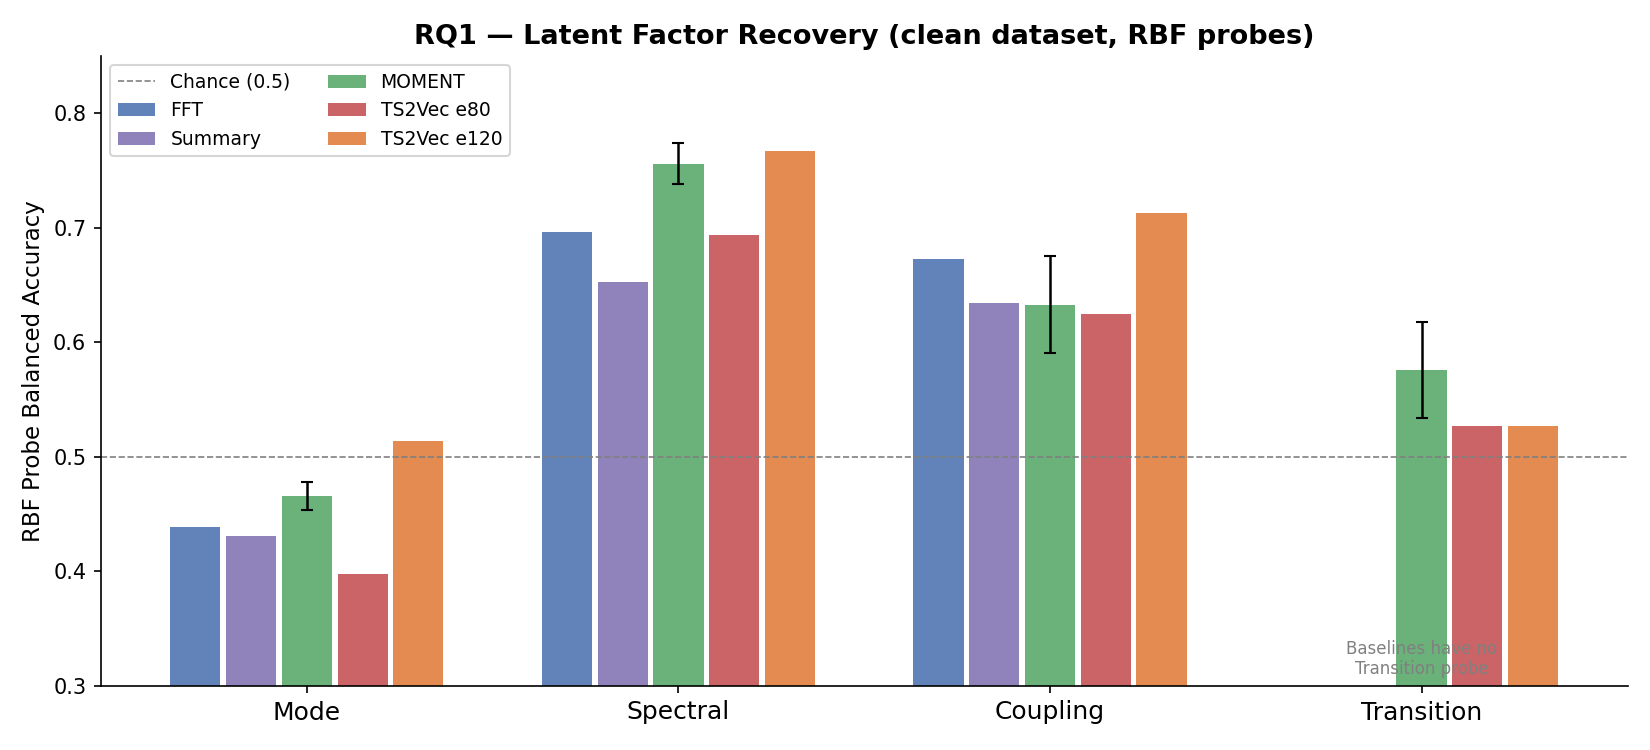
\includegraphics[width=\linewidth]{figures/fig1_rq1_probes.png}
\caption{RQ1 probe accuracy}
\end{figure}

\begin{longtable}{|l|l|l|l|l|l|}
\hline
\textbf{Method} & \textbf{Mode} & \textbf{Spectral} & \textbf{Coupling} & \textbf{Transition} & \textbf{Load R$^2$} \\
\hline
\endfirsthead
\hline
\textbf{Method} & \textbf{Mode} & \textbf{Spectral} & \textbf{Coupling} & \textbf{Transition} & \textbf{Load R$^2$} \\
\hline
\endhead
\hline
\endfoot
FFT baseline & 0.439 & 0.696 & 0.673 & --- & $-$0.006 \\
\hline
Summary baseline & 0.431 & 0.653 & 0.634 & --- & $-$0.006 \\
\hline
MOMENT & 0.466 $\pm$0.012 & 0.756 $\pm$0.018 & 0.633 $\pm$0.042 & 0.576 $\pm$0.042 & $-$0.037 $\pm$0.049 \\
\hline
TS2Vec e80 & 0.398 & 0.694 & 0.625 & 0.527 & $-$0.006 \\
\hline
\textbf{TS2Vec e120} & \textbf{0.514} & \textbf{0.767} & \textbf{0.713} & 0.527 & $-$0.006 \\
\hline
\end{longtable}

\subsubsection{7.2 Average Balanced Accuracy (mode + spectral + coupling)}

\begin{figure}[H]
\centering
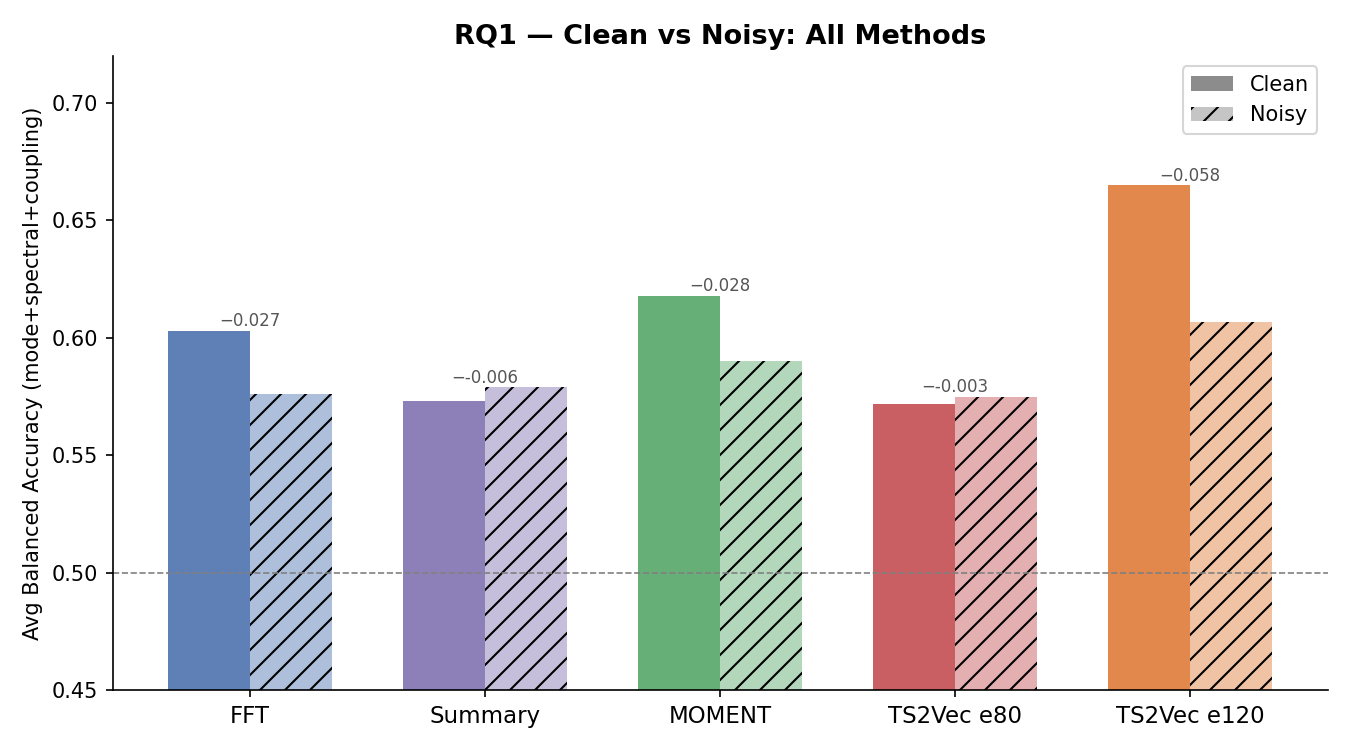
\includegraphics[width=\linewidth]{figures/fig2_rq1_clean_noisy.png}
\caption{Clean vs noisy comparison}
\end{figure}

\begin{longtable}{|l|l|l|l|}
\hline
\textbf{Method} & \textbf{Clean} & \textbf{Noisy} & \textbf{Drop} \\
\hline
\endfirsthead
\hline
\textbf{Method} & \textbf{Clean} & \textbf{Noisy} & \textbf{Drop} \\
\hline
\endhead
\hline
\endfoot
FFT baseline & 0.603 & 0.576 & $-$0.027 \\
\hline
Summary baseline & 0.573 & 0.579 & +0.006 \\
\hline
MOMENT & 0.618 & 0.590 & $-$0.028 \\
\hline
TS2Vec e80 & 0.572 & 0.575 & +0.003 \\
\hline
\textbf{TS2Vec e120} & \textbf{0.665} & \textbf{0.607} & $-$0.058 \\
\hline
\end{longtable}

The margin of the best learned method over the best baseline is only \textbf{+6.2 pp} on clean data,
narrowing to \textbf{+3.1 pp} on noisy data.

\subsubsection{7.3 Clustering ARI (K-Means, clean dataset)}

\begin{figure}[H]
\centering
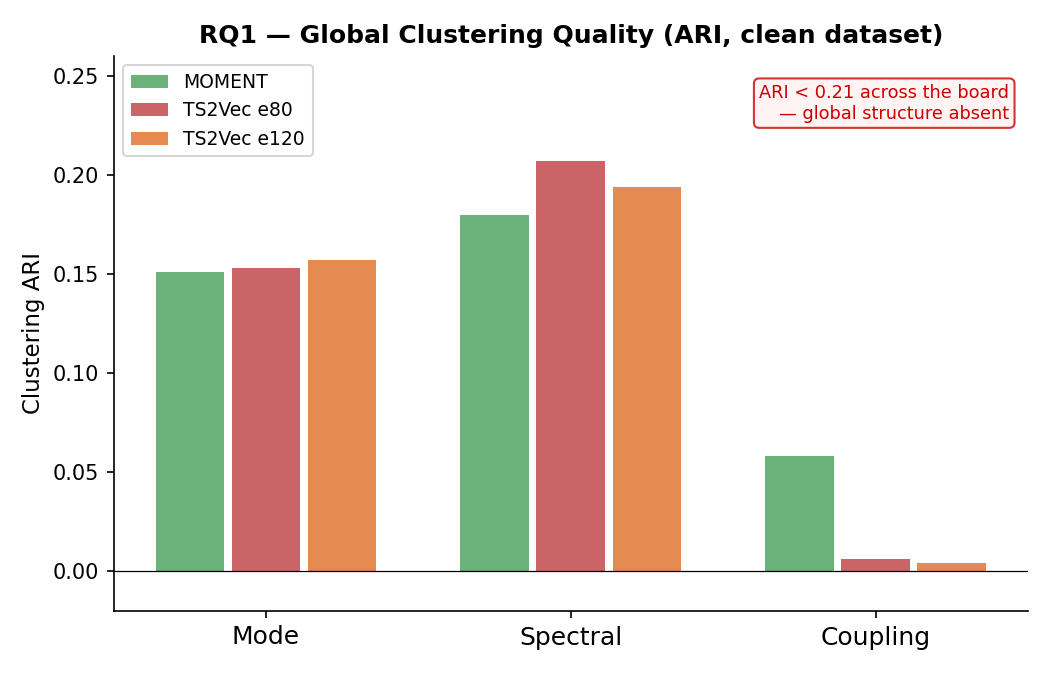
\includegraphics[width=\linewidth]{figures/fig3_rq1_clustering.png}
\caption{Clustering ARI}
\end{figure}

\begin{longtable}{|l|l|l|l|l|}
\hline
\textbf{Method} & \textbf{Mode} & \textbf{Spectral} & \textbf{Coupling} & \textbf{Avg} \\
\hline
\endfirsthead
\hline
\textbf{Method} & \textbf{Mode} & \textbf{Spectral} & \textbf{Coupling} & \textbf{Avg} \\
\hline
\endhead
\hline
\endfoot
MOMENT & 0.151 & 0.180 & 0.058 & 0.130 \\
\hline
TS2Vec e80 & 0.153 & 0.207 & 0.006 & 0.122 \\
\hline
TS2Vec e120 & 0.157 & 0.194 & 0.004 & 0.118 \\
\hline
\end{longtable}

Global clustering quality is uniformly poor (ARI < 0.21). More training (e80$\rightarrow$e120) helps probes
but \textbf{degrades} coupling clustering. Load R$^2$ $\leq$ 0 for every method in every setting.

\vspace{4pt}\hrule\vspace{4pt}

\subsection{8. RQ2 --- Trace Geometry Results}

\subsubsection{8.1 Full Metric Table}

\begin{figure}[H]
\centering
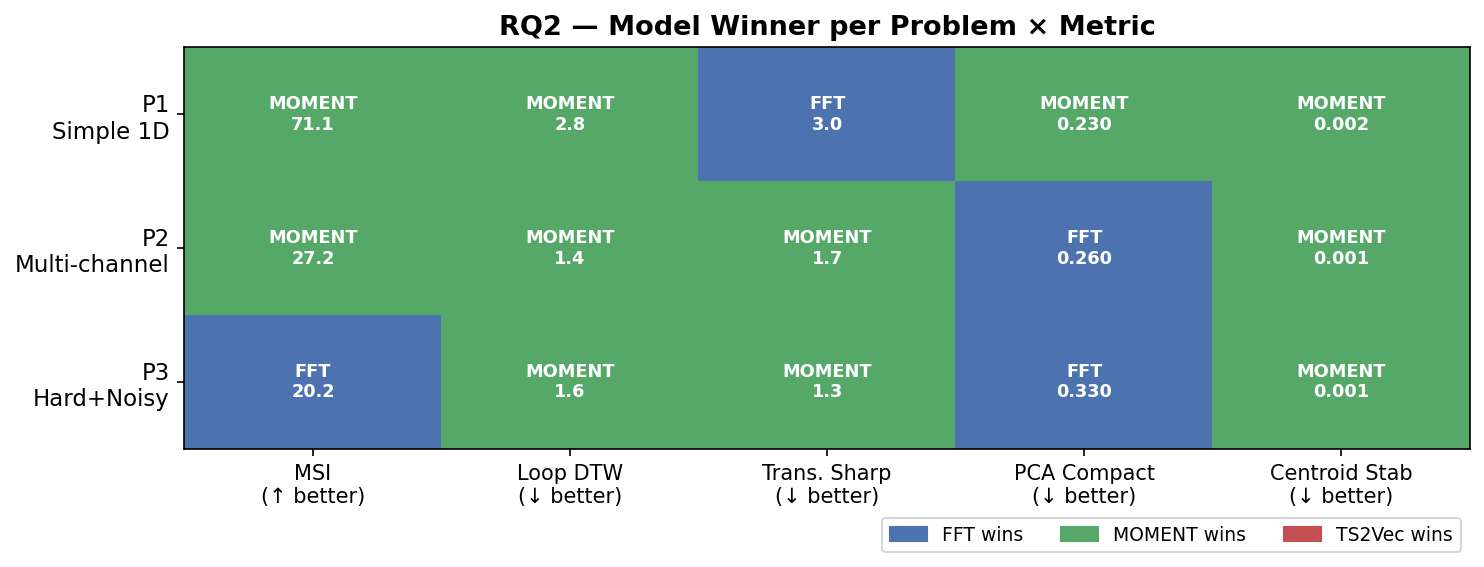
\includegraphics[width=\linewidth]{figures/fig4_rq2_winner_heatmap.png}
\caption{Winner heatmap}
\end{figure}

\begin{longtable}{|l|l|l|l|l|l|}
\hline
\textbf{} & \textbf{MSI $\uparrow$} & \textbf{Loop DTW $\downarrow$} & \textbf{Trans. Sharp $\downarrow$} & \textbf{PCA Compact $\downarrow$} & \textbf{Centroid Stab $\downarrow$} \\
\hline
\endfirsthead
\hline
\textbf{} & \textbf{MSI $\uparrow$} & \textbf{Loop DTW $\downarrow$} & \textbf{Trans. Sharp $\downarrow$} & \textbf{PCA Compact $\downarrow$} & \textbf{Centroid Stab $\downarrow$} \\
\hline
\endhead
\hline
\endfoot
P1 / FFT & 11.1 & 66.6 & \textbf{3.0} & 0.50 & 0.289 \\
\hline
P1 / MOMENT & \textbf{71.1} & \textbf{2.76} & 5.7 & \textbf{0.23} & \textbf{0.002} \\
\hline
P1 / TS2Vec & 20.0 & 44.6 & 3.0 & 0.37 & 0.085 \\
\hline
P2 / FFT & 22.5 & 146.1 & 3.3 & \textbf{0.26} & 0.278 \\
\hline
P2 / MOMENT & \textbf{27.2} & \textbf{1.43} & \textbf{1.67} & 1.63 & \textbf{0.001} \\
\hline
P2 / TS2Vec & 4.4 & 108.2 & 3.67 & 48.4 & 0.509 \\
\hline
P3 / FFT & \textbf{20.2} & 167.4 & 4.0 & \textbf{0.33} & 0.364 \\
\hline
P3 / MOMENT & 14.3 & \textbf{1.64} & \textbf{1.33} & 7.97 & \textbf{0.001} \\
\hline
P3 / TS2Vec & 4.6 & 107.8 & 4.0 & 55.9 & 0.529 \\
\hline
\end{longtable}

\begin{figure}[H]
\centering
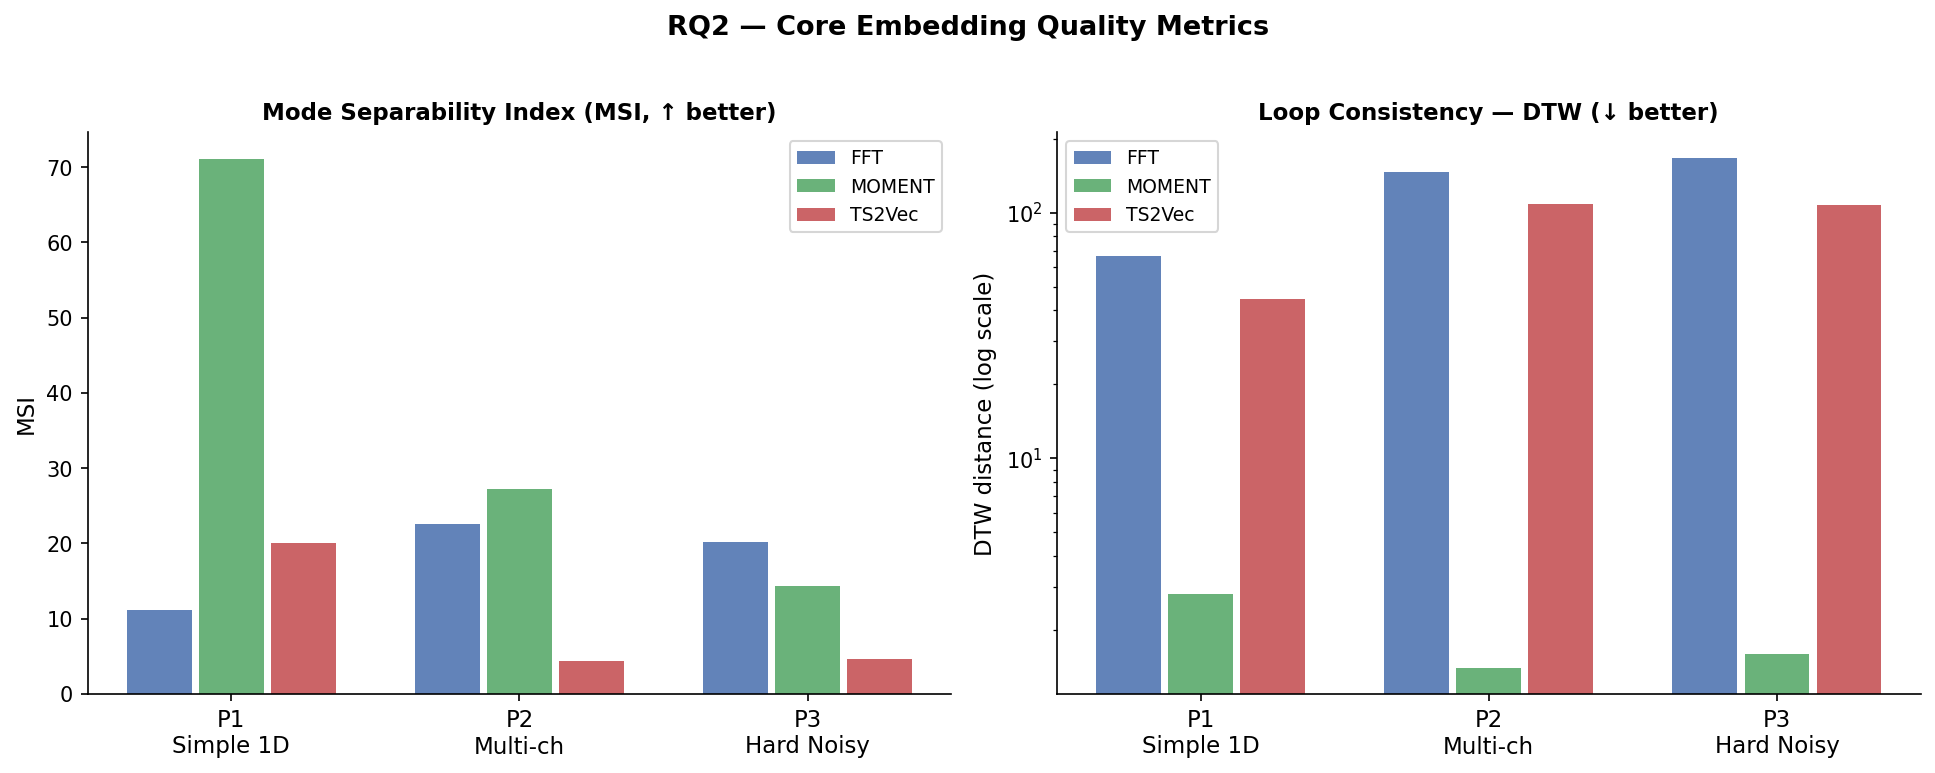
\includegraphics[width=\linewidth]{figures/fig5_rq2_msi_loop.png}
\caption{MSI and Loop Consistency}
\end{figure}

\begin{figure}[H]
\centering
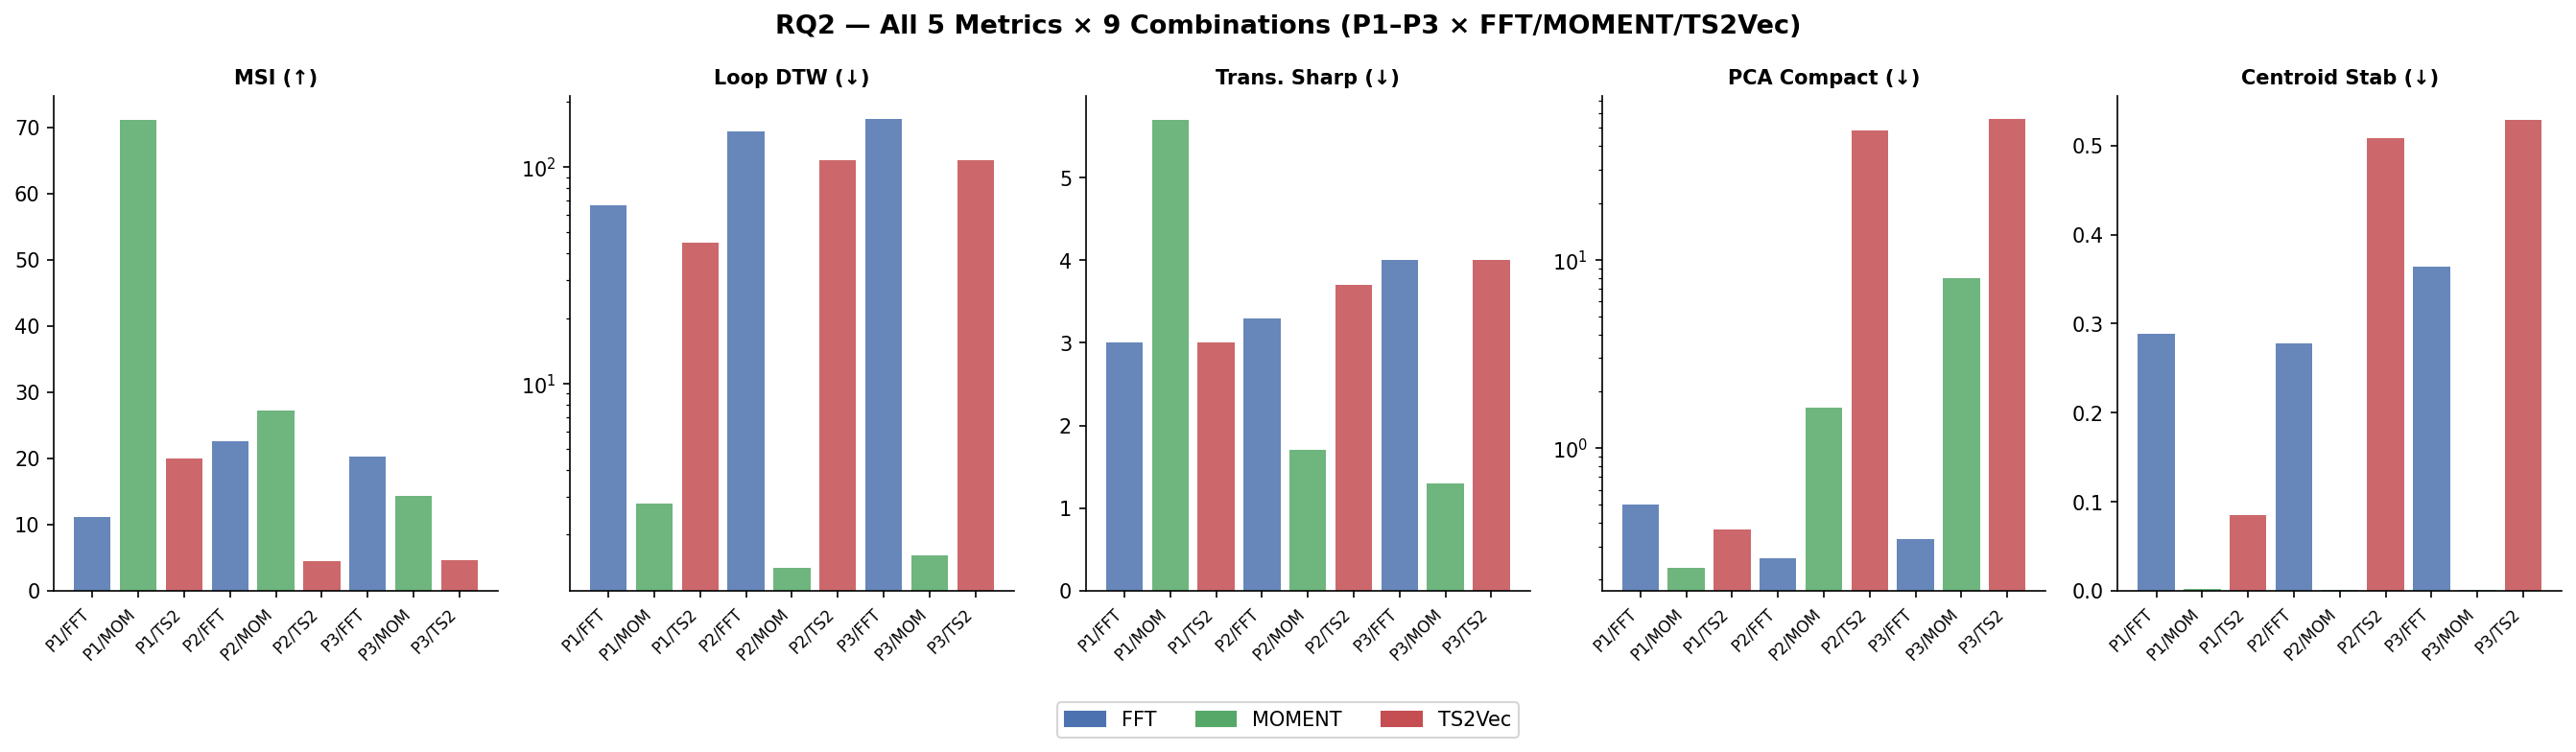
\includegraphics[width=\linewidth]{figures/fig8_rq2_all_metrics.png}
\caption{All 5 metrics}
\end{figure}

\begin{figure}[H]
\centering
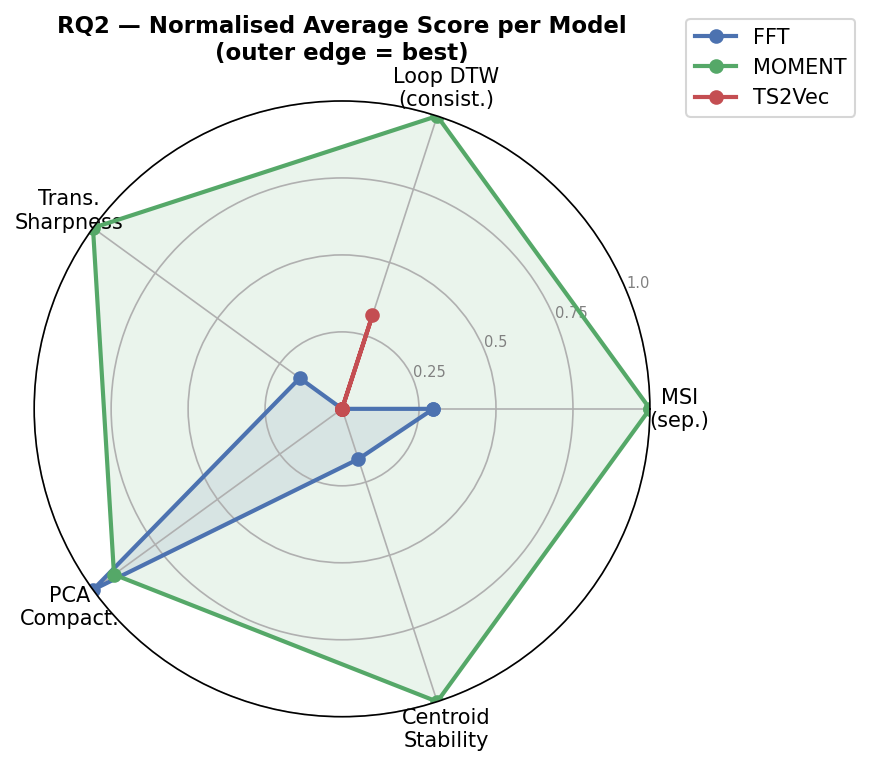
\includegraphics[width=\linewidth]{figures/fig6_rq2_radar.png}
\caption{Radar chart}
\end{figure}

\subsubsection{8.2 Key Findings}

\textbf{MOMENT's loop consistency is extraordinary.} Loop DTW of 1.4--2.8 across all three problems,
vs 66--167 for FFT and 44--108 for TS2Vec --- roughly 20--100× better. Mode traces form tight,
repeatable closed orbits.

\textbf{MOMENT centroid stability is near-zero.} 0.001--0.002 vs 0.08--0.53 for others. Mode regions
don't drift between test trajectories --- critical for reference-based anomaly detection.

\textbf{FFT beats MOMENT on MSI in the hard noisy case (P3): 20.2 vs 14.3.} When frequencies are
close and noise is high, the raw spectrum remains more discriminative than the pretrained features.
MOMENT still wins on loop consistency and transition sharpness even in P3.

\textbf{TS2Vec is consistently the worst.} Low MSI (4.4--20.0), catastrophic PCA compactness on
multichannel (48--56), centroid stability 0.09--0.53. The 64-dim trained representation fails to
find useful geometry in these problems.

\vspace{4pt}\hrule\vspace{4pt}

\subsection{9. RQ3 --- Landscape Sweep Results}

\subsubsection{9.1 Noise Axis ($\sigma$ ∈ \{0.00, 0.20, 0.40\})}

\begin{longtable}{|l|l|l|l|l|l|}
\hline
\textbf{Scenario} & \textbf{Model} & \textbf{MSI $\uparrow$} & \textbf{Sil $\uparrow$} & \textbf{Loop DTW $\downarrow$} & \textbf{Centroid Stab $\downarrow$} \\
\hline
\endfirsthead
\hline
\textbf{Scenario} & \textbf{Model} & \textbf{MSI $\uparrow$} & \textbf{Sil $\uparrow$} & \textbf{Loop DTW $\downarrow$} & \textbf{Centroid Stab $\downarrow$} \\
\hline
\endhead
\hline
\endfoot
noise\_000 & fft32 & 37.2 & 0.394 & 147.0 & 0.367 \\
\hline
noise\_000 & fft8 & 21.4 & 0.398 & 144.6 & 0.605 \\
\hline
noise\_000 & moment & \textbf{73.1} & \textbf{0.501} & \textbf{5.2} & \textbf{0.008} \\
\hline
noise\_020 & fft32 & 31.5 & 0.410 & 141.0 & 0.481 \\
\hline
noise\_020 & fft8 & 20.6 & 0.428 & 138.7 & 0.656 \\
\hline
noise\_020 & moment & \textbf{67.7} & \textbf{0.469} & \textbf{5.3} & \textbf{0.008} \\
\hline
noise\_040 & fft32 & 22.8 & 0.328 & 175.7 & 0.725 \\
\hline
noise\_040 & fft8 & 17.2 & 0.365 & 171.0 & 0.873 \\
\hline
noise\_040 & moment & \textbf{59.9} & \textbf{0.417} & \textbf{5.6} & \textbf{0.009} \\
\hline
\end{longtable}

MOMENT's MSI drops from 73.1 to 59.9 over the full noise range ($-$13.2 pp), while FFT32
drops from 37.2 to 22.8 ($-$14.4 pp). Both degrade similarly in absolute terms, but MOMENT
\textbf{maintains a consistent 37+ point lead} throughout. Loop DTW is essentially constant for MOMENT
(5.2--5.6) regardless of noise --- the orbit consistency is noise-invariant.

\subsubsection{9.2 Missing Data Axis}

\begin{longtable}{|l|l|l|l|l|l|}
\hline
\textbf{Scenario} & \textbf{Model} & \textbf{MSI $\uparrow$} & \textbf{Sil $\uparrow$} & \textbf{Loop DTW $\downarrow$} & \textbf{Centroid Stab $\downarrow$} \\
\hline
\endfirsthead
\hline
\textbf{Scenario} & \textbf{Model} & \textbf{MSI $\uparrow$} & \textbf{Sil $\uparrow$} & \textbf{Loop DTW $\downarrow$} & \textbf{Centroid Stab $\downarrow$} \\
\hline
\endhead
\hline
\endfoot
miss\_rand10 & fft32 & 29.0 & 0.391 & 132.1 & 0.410 \\
\hline
miss\_rand10 & fft8 & 19.8 & 0.414 & 128.7 & 0.567 \\
\hline
miss\_rand10 & moment & \textbf{65.0} & \textbf{0.446} & \textbf{5.5} & \textbf{0.008} \\
\hline
miss\_rand30 & fft32 & 20.6 & 0.329 & 110.6 & 0.430 \\
\hline
miss\_rand30 & fft8 & 16.3 & 0.383 & 106.5 & 0.517 \\
\hline
miss\_rand30 & moment & \textbf{47.8} & \textbf{0.318} & \textbf{6.5} & \textbf{0.009} \\
\hline
miss\_block30 & fft32 & 24.2 & 0.303 & 148.5 & 0.417 \\
\hline
miss\_block30 & fft8 & 14.7 & 0.310 & 146.1 & 0.679 \\
\hline
miss\_block30 & moment & \textbf{40.4} & \textbf{0.294} & \textbf{8.9} & \textbf{0.016} \\
\hline
miss\_channel & fft32 & 13.5 & 0.106 & 478.1 & 0.850 \\
\hline
miss\_channel & fft8 & 7.1 & 0.106 & 476.6 & 1.591 \\
\hline
miss\_channel & moment & --- & --- & --- & --- \\
\hline
\end{longtable}

\textbf{Random dropout} is relatively benign for MOMENT (rand10: 65.0, rand30: 47.8 vs baseline 72.5).
\textbf{Block dropout} is harder --- the contiguous gap disrupts the local temporal context that MOMENT
relies on (block30: 40.4, $-$32.1 pp from baseline).
\textbf{Channel dropout} is catastrophic for FFT (MSI 13.5, loop DTW 478) and was not measurable for
MOMENT (zero-padded channel produces degenerate embeddings). This is a key production risk: any
sensor outage breaks the FFT's spectral decomposition entirely.

\subsubsection{9.3 Number of Modes Axis}

\begin{longtable}{|l|l|l|l|l|l|}
\hline
\textbf{Scenario} & \textbf{Model} & \textbf{MSI $\uparrow$} & \textbf{Sil $\uparrow$} & \textbf{Loop DTW $\downarrow$} & \textbf{Centroid Stab $\downarrow$} \\
\hline
\endfirsthead
\hline
\textbf{Scenario} & \textbf{Model} & \textbf{MSI $\uparrow$} & \textbf{Sil $\uparrow$} & \textbf{Loop DTW $\downarrow$} & \textbf{Centroid Stab $\downarrow$} \\
\hline
\endhead
\hline
\endfoot
modes\_2 & fft32 & 43.0 & 0.426 & 114.2 & 0.212 \\
\hline
modes\_2 & moment & \textbf{83.2} & \textbf{0.599} & \textbf{4.9} & \textbf{0.005} \\
\hline
modes\_5 & fft32 & 33.3 & 0.335 & 147.4 & 0.521 \\
\hline
modes\_5 & moment & \textbf{61.2} & \textbf{0.317} & \textbf{5.1} & \textbf{0.010} \\
\hline
modes\_8 & fft32 & 30.9 & 0.250 & 143.2 & 0.550 \\
\hline
modes\_8 & moment & \textbf{52.2} & \textbf{0.146} & \textbf{5.7} & \textbf{0.011} \\
\hline
\end{longtable}

As the number of modes increases, both methods degrade monotonically, but MOMENT's gap over FFT
grows: at K=2 it is +40.2 pp; at K=8 it is +21.4 pp. Silhouette scores converge --- MOMENT's
silhouette advantage disappears at K=8 (0.146 vs 0.250) because projecting many modes into 2
PCA dimensions forces overlap. Loop DTW for MOMENT remains stable (4.9--5.7) regardless of K,
while FFT loop DTW also stays flat (\textasciitilde{}115--147) --- mode count doesn't affect trace consistency.

\subsubsection{9.4 Signal Type Axis}

\begin{longtable}{|l|l|l|l|l|l|}
\hline
\textbf{Scenario} & \textbf{Model} & \textbf{MSI $\uparrow$} & \textbf{Sil $\uparrow$} & \textbf{Loop DTW $\downarrow$} & \textbf{Centroid Stab $\downarrow$} \\
\hline
\endfirsthead
\hline
\textbf{Scenario} & \textbf{Model} & \textbf{MSI $\uparrow$} & \textbf{Sil $\uparrow$} & \textbf{Loop DTW $\downarrow$} & \textbf{Centroid Stab $\downarrow$} \\
\hline
\endhead
\hline
\endfoot
baseline (sine) & fft32 & 37.1 & 0.407 & 141.9 & 0.371 \\
\hline
baseline (sine) & moment & \textbf{72.5} & \textbf{0.497} & \textbf{5.2} & \textbf{0.008} \\
\hline
sig\_mixed & fft32 & 22.6 & 0.212 & 280.7 & 0.436 \\
\hline
sig\_mixed & moment & \textbf{36.9} & \textbf{0.184} & \textbf{8.8} & \textbf{0.008} \\
\hline
sig\_event & fft32 & \textbf{23.9} & \textbf{0.208} & 252.2 & 0.620 \\
\hline
sig\_event & moment & 18.7 & 0.038 & \textbf{11.1} & \textbf{0.012} \\
\hline
sig\_step & fft32 & \textbf{9.6} & $-$0.020 & 274.4 & 0.447 \\
\hline
sig\_step & moment & 2.8 & $-$0.011 & \textbf{10.4} & \textbf{0.011} \\
\hline
\end{longtable}

\textbf{This is the most consequential finding of RQ3.} Both methods are built around spectral
assumptions --- MOMENT is pretrained on smooth continuous signals; FFT explicitly computes frequency
content. When the signal type changes to steps or events, \textbf{FFT beats MOMENT on MSI} (step: 9.6
vs 2.8; event: 23.9 vs 18.7). MOMENT's pretrained features are essentially blind to the
distinguishing information in non-periodic signals.

However, MOMENT retains its loop consistency advantage even on step/event signals (loop DTW \textasciitilde{}10--11
vs FFT \textasciitilde{}250--274). The mode orbits are still compact --- they just overlap in PCA space.

\vspace{4pt}\hrule\vspace{4pt}

\subsection{10. RQ4 --- CNC-Analogous Benchmark Results}

\subsubsection{10.1 Program Step Labels}

\begin{longtable}{|l|l|l|l|l|l|l|}
\hline
\textbf{Scenario} & \textbf{Model} & \textbf{MSI $\uparrow$} & \textbf{Sil $\uparrow$} & \textbf{Loop DTW $\downarrow$} & \textbf{Trans. Sharp $\downarrow$} & \textbf{Centroid Stab $\downarrow$} \\
\hline
\endfirsthead
\hline
\textbf{Scenario} & \textbf{Model} & \textbf{MSI $\uparrow$} & \textbf{Sil $\uparrow$} & \textbf{Loop DTW $\downarrow$} & \textbf{Trans. Sharp $\downarrow$} & \textbf{Centroid Stab $\downarrow$} \\
\hline
\endhead
\hline
\endfoot
cnc\_part\_simple & fft & 55.9 & 0.002 & 166.2 & 2.74 & 0.897 \\
\hline
cnc\_part\_simple & moment & 36.1 & $-$0.008 & \textbf{2.89} & 2.11 & \textbf{0.004} \\
\hline
cnc\_part\_full & fft & \textbf{68.2} & \textbf{0.030} & 197.0 & 2.09 & 0.776 \\
\hline
cnc\_part\_full & moment & 43.7 & $-$0.009 & \textbf{2.29} & 1.51 & \textbf{0.003} \\
\hline
cnc\_two\_parts & fft & 45.0 & $-$0.024 & 837.4 & 1.16 & 1.517 \\
\hline
cnc\_two\_parts & moment & \textbf{42.7} & $-$0.036 & \textbf{2.97} & 1.21 & \textbf{0.003} \\
\hline
cnc\_tool\_wear & fft & \textbf{64.6} & \textbf{0.018} & 354.1 & 2.13 & 0.969 \\
\hline
cnc\_tool\_wear & moment & 43.3 & $-$0.010 & \textbf{2.26} & 1.37 & \textbf{0.003} \\
\hline
cnc\_noisy & fft & \textbf{65.1} & \textbf{0.021} & 240.7 & 2.17 & 0.846 \\
\hline
cnc\_noisy & moment & 43.1 & $-$0.006 & \textbf{2.27} & 1.28 & \textbf{0.003} \\
\hline
cnc\_pocket & fft & \textbf{81.5} & nan & 243.2 & 3.06 & 0.829 \\
\hline
cnc\_pocket & moment & 54.9 & nan & \textbf{2.25} & 1.54 & \textbf{0.002} \\
\hline
cnc\_faults & fft & \textbf{51.1} & \textbf{0.022} & 244.3 & 1.83 & 1.096 \\
\hline
cnc\_faults & moment & 38.8 & $-$0.004 & \textbf{2.02} & 1.14 & \textbf{0.003} \\
\hline
\end{longtable}

\subsubsection{10.2 Operating State Labels}

\begin{longtable}{|l|l|l|l|l|l|l|}
\hline
\textbf{Scenario} & \textbf{Model} & \textbf{MSI $\uparrow$} & \textbf{Sil $\uparrow$} & \textbf{Loop DTW $\downarrow$} & \textbf{Trans. Sharp $\downarrow$} & \textbf{Centroid Stab $\downarrow$} \\
\hline
\endfirsthead
\hline
\textbf{Scenario} & \textbf{Model} & \textbf{MSI $\uparrow$} & \textbf{Sil $\uparrow$} & \textbf{Loop DTW $\downarrow$} & \textbf{Trans. Sharp $\downarrow$} & \textbf{Centroid Stab $\downarrow$} \\
\hline
\endhead
\hline
\endfoot
cnc\_part\_simple & fft & 40.9 & \textbf{0.509} & 370.1 & 1.50 & 1.228 \\
\hline
cnc\_part\_simple & moment & 37.6 & 0.098 & \textbf{6.85} & 2.50 & \textbf{0.004} \\
\hline
cnc\_part\_full & fft & 48.2 & \textbf{0.446} & 417.2 & 2.50 & 1.074 \\
\hline
cnc\_part\_full & moment & 44.3 & 0.170 & \textbf{5.38} & 2.50 & \textbf{0.003} \\
\hline
cnc\_two\_parts & fft & 39.3 & \textbf{0.346} & 2214.2 & 2.50 & 1.658 \\
\hline
cnc\_two\_parts & moment & \textbf{41.0} & 0.123 & \textbf{7.06} & 2.50 & \textbf{0.004} \\
\hline
cnc\_tool\_wear & fft & 47.0 & \textbf{0.429} & 825.3 & 2.50 & 1.216 \\
\hline
cnc\_tool\_wear & moment & 43.8 & 0.164 & \textbf{5.30} & 2.50 & \textbf{0.003} \\
\hline
cnc\_noisy & fft & 47.5 & \textbf{0.443} & 475.3 & 2.50 & 1.099 \\
\hline
cnc\_noisy & moment & 44.1 & 0.153 & \textbf{5.30} & 2.50 & \textbf{0.003} \\
\hline
cnc\_pocket & fft & 55.3 & \textbf{0.482} & 581.3 & 1.67 & 1.360 \\
\hline
cnc\_pocket & moment & \textbf{55.8} & 0.241 & \textbf{5.69} & 2.33 & \textbf{0.003} \\
\hline
cnc\_faults & fft & 35.1 & \textbf{0.412} & 498.3 & 2.67 & 1.510 \\
\hline
cnc\_faults & moment & 38.6 & 0.149 & \textbf{3.99} & 2.00 & \textbf{0.003} \\
\hline
\end{longtable}

\subsubsection{10.3 Key Findings}

\textbf{FFT dominates program-step MSI.} Across all 7 scenarios, FFT32 achieves 45--82 MSI vs MOMENT's
36--55. The spectral structure of the machining signals (spindle frequency, vibration harmonics)
carries strong mode-separating information that FFT captures directly.

\textbf{MOMENT dominates geometry.} Loop DTW 2.0--2.9 (MOMENT) vs 166--837 (FFT) for program steps;
5.4--7.1 (MOMENT) vs 370--2214 (FFT) for operating states. The 100--300× gap is consistent
across all scenarios including noisy and fault-injected ones.

\textbf{Operating state is easier than program step.} FFT silhouette on op-state (0.35--0.51) is far
higher than on program step (\textasciitilde{}0.0--0.03). Op-states correspond to coarse machine behaviours
(cutting vs. idle vs. homing) that produce clearly distinct spectral signatures; program steps
within a cutting phase share similar spectra but differ in toolpath position.

\textbf{MOMENT wins on op-state MSI in cnc\_pocket (55.8 vs 55.3) and cnc\_faults (38.6 vs 35.1).}
For the most complex scenario (11 program steps with Z-varying geometry) and the fault-injected
scenario, MOMENT's feature richness starts to matter for MSI as well. This hints that MOMENT's
768-dim representation captures more than spectral amplitude.

\textbf{Discrete channels (tool\_id, alarm\_code) do not break MOMENT.} MOMENT's mean-pooling across
channels treats discrete channels the same as continuous ones. The embedding quality on
cnc\_faults (which has active alarm codes in 8\% of windows) is comparable to clean scenarios.

\vspace{4pt}\hrule\vspace{4pt}

\subsection{11. RQ5 --- Window Size Sweep Results}

\subsubsection{11.1 Program Step Labels}

\begin{longtable}{|l|l|l|l|l|l|l|l|}
\hline
\textbf{Window} & \textbf{Stride} & \textbf{Model} & \textbf{MSI $\uparrow$} & \textbf{Sil $\uparrow$} & \textbf{Loop DTW $\downarrow$} & \textbf{Trans. Sharp $\downarrow$} & \textbf{Centroid Stab $\downarrow$} \\
\hline
\endfirsthead
\hline
\textbf{Window} & \textbf{Stride} & \textbf{Model} & \textbf{MSI $\uparrow$} & \textbf{Sil $\uparrow$} & \textbf{Loop DTW $\downarrow$} & \textbf{Trans. Sharp $\downarrow$} & \textbf{Centroid Stab $\downarrow$} \\
\hline
\endhead
\hline
\endfoot
32 & 4 & fft & 48.9 & 0.018 & 118.1 & 2.00 & 0.087 \\
\hline
32 & 4 & moment & 37.9 & 0.038 & \textbf{3.71} & 2.47 & \textbf{0.001} \\
\hline
\textbf{64} & \textbf{8} & \textbf{fft} & \textbf{64.3} & \textbf{0.057} & 144.0 & 1.93 & 0.335 \\
\hline
\textbf{64} & \textbf{8} & \textbf{moment} & \textbf{48.6} & \textbf{0.065} & \textbf{1.98} & \textbf{1.15} & \textbf{0.002} \\
\hline
128 & 16 & fft & 50.0 & $-$0.021 & 197.6 & 3.40 & 0.667 \\
\hline
128 & 16 & moment & 35.9 & 0.021 & 2.00 & 2.22 & 0.003 \\
\hline
256 & 32 & fft & 39.0 & 0.258 & 199.5 & 1.11 & 1.538 \\
\hline
256 & 32 & moment & 28.5 & 0.033 & 0.92 & 1.26 & 0.003 \\
\hline
512 & 64 & fft & 18.5 & $-$0.073 & 664.6 & 1.71 & 12.049 \\
\hline
512 & 64 & moment & 28.0 & $-$0.096 & 1.25 & 1.76 & 0.006 \\
\hline
\end{longtable}

\subsubsection{11.2 Operating State Labels}

\begin{longtable}{|l|l|l|l|l|l|l|l|}
\hline
\textbf{Window} & \textbf{Stride} & \textbf{Model} & \textbf{MSI $\uparrow$} & \textbf{Sil $\uparrow$} & \textbf{Loop DTW $\downarrow$} & \textbf{Trans. Sharp $\downarrow$} & \textbf{Centroid Stab $\downarrow$} \\
\hline
\endfirsthead
\hline
\textbf{Window} & \textbf{Stride} & \textbf{Model} & \textbf{MSI $\uparrow$} & \textbf{Sil $\uparrow$} & \textbf{Loop DTW $\downarrow$} & \textbf{Trans. Sharp $\downarrow$} & \textbf{Centroid Stab $\downarrow$} \\
\hline
\endhead
\hline
\endfoot
32 & 4 & fft & 35.4 & 0.357 & 199.3 & 2.39 & 0.076 \\
\hline
32 & 4 & moment & 34.8 & 0.127 & \textbf{6.84} & 1.70 & \textbf{0.001} \\
\hline
\textbf{64} & \textbf{8} & \textbf{fft} & \textbf{55.3} & \textbf{0.477} & 247.1 & \textbf{1.40} & 0.341 \\
\hline
\textbf{64} & \textbf{8} & \textbf{moment} & \textbf{46.3} & \textbf{0.213} & \textbf{3.67} & 1.07 & \textbf{0.002} \\
\hline
128 & 16 & fft & 62.7 & 0.470 & 648.0 & 3.00 & 0.924 \\
\hline
128 & 16 & moment & 50.6 & 0.203 & 7.51 & 3.00 & 0.003 \\
\hline
256 & 32 & fft & 0.0 & nan & 692.5 & nan & 0.840 \\
\hline
256 & 32 & moment & 0.0 & nan & 3.46 & nan & 0.002 \\
\hline
512 & 64 & fft & 0.0 & nan & 658.5 & nan & 2.971 \\
\hline
512 & 64 & moment & 0.0 & nan & 1.12 & nan & 0.003 \\
\hline
\end{longtable}

\subsubsection{11.3 Key Findings}

\textbf{The sweet spot is ws=64 for both models.} FFT reaches its peak program-step MSI (64.3) and
op-state silhouette (0.477) at ws=64. MOMENT peaks at ws=64 for program-step (MSI=48.6,
silhouette=0.065) and for op-state (MSI=46.3, silhouette=0.213).

\textbf{FFT collapses at ws=512.} MSI drops from 64.3 at ws=64 to 18.5 at ws=512 for program steps.
The centroid stability explodes to 12.0 --- mode regions drift massively at very large windows.
At ws=512 with stride=64, there are only \textasciitilde{}106 windows per trajectory, breaking the statistical
reliability of the metrics.

\textbf{MOMENT is more robust at large windows.} At ws=512, MOMENT MSI (28.0) beats FFT (18.5) for
program steps. MOMENT also achieves its best loop DTW at ws=512 (1.25) --- because at 512
samples the window naturally covers an entire mode segment, making successive visits nearly
identical.

\textbf{Op-state metrics collapse at ws$\geq$256.} Both models show MSI=0 and NaN silhouette. At stride=32,
the very short RAPID and HOMING segments produce fewer than one window in some trajectories,
so op-state coverage becomes incomplete. This is a real production constraint: window size
must be small relative to the shortest mode duration.

\textbf{MOMENT padding penalty is invisible at ws=64.} Despite 7× zero-padding (64 $\rightarrow$ 512), MOMENT
performs well --- the zero-padding is right-sided and the signal is left-aligned, so the first
64 samples are unaffected. The penalty only appears at ws=32 where 15× padding dilutes the
signal substantially.

\vspace{4pt}\hrule\vspace{4pt}

\subsection{12. RQ6 --- Signal Ablation Results}

\subsubsection{12.1 Step Channel Ratio (ratio\_0step $\rightarrow$ ratio\_4step)}

\begin{longtable}{|l|l|l|l|l|l|l|}
\hline
\textbf{Scenario} & \textbf{Step ch} & \textbf{Model} & \textbf{MSI $\uparrow$} & \textbf{Sil $\uparrow$} & \textbf{Loop DTW $\downarrow$} & \textbf{Centroid Stab $\downarrow$} \\
\hline
\endfirsthead
\hline
\textbf{Scenario} & \textbf{Step ch} & \textbf{Model} & \textbf{MSI $\uparrow$} & \textbf{Sil $\uparrow$} & \textbf{Loop DTW $\downarrow$} & \textbf{Centroid Stab $\downarrow$} \\
\hline
\endhead
\hline
\endfoot
ratio\_0step & 0/4 & fft32 & 38.3 & 0.441 & --- & 0.311 \\
\hline
ratio\_0step & 0/4 & moment & \textbf{82.8} & \textbf{0.429} & --- & \textbf{0.002} \\
\hline
ratio\_1step & 1/4 & fft32 & 28.1 & 0.297 & --- & 0.388 \\
\hline
ratio\_1step & 1/4 & moment & \textbf{73.4} & \textbf{0.382} & --- & \textbf{0.002} \\
\hline
ratio\_2step & 2/4 & fft32 & 22.4 & 0.208 & --- & --- \\
\hline
ratio\_2step & 2/4 & moment & \textbf{60.2} & \textbf{0.293} & --- & \textbf{0.002} \\
\hline
ratio\_3step & 3/4 & fft32 & 17.0 & 0.128 & --- & --- \\
\hline
ratio\_3step & 3/4 & moment & \textbf{48.1} & \textbf{0.182} & --- & \textbf{0.002} \\
\hline
ratio\_4step & 4/4 & fft32 & 9.6 & $-$0.020 & --- & --- \\
\hline
ratio\_4step & 4/4 & moment & \textbf{27.7} & \textbf{0.085} & --- & \textbf{0.002} \\
\hline
\end{longtable}

\textbf{MOMENT degrades gracefully; FFT collapses.} Each additional step channel costs FFT32
roughly 7 MSI points (38.3 $\rightarrow$ 9.6, $-$75\%). MOMENT loses about 14 MSI points per step channel
added (82.8 $\rightarrow$ 27.7, $-$67\%) but remains substantially ahead in absolute terms at every level.
At ratio\_4step, MOMENT MSI (27.7) is 3× FFT (9.6).

\textbf{The RQ3 sig\_step result (MOMENT 2.8, FFT 9.6) was a worst-case boundary.} In RQ3, the step
signal was designed with abrupt transitions that share identical amplitude histograms across modes
--- a pathological case where even the signal envelope carries no discriminating information. RQ6's
step channels use natural step levels tied to mode identity, which MOMENT can partially exploit via
temporal context.

\textbf{Silhouette tracks MSI.} At ratio\_4step, FFT32 silhouette goes negative ($-$0.020), confirming
that clusters overlap in PCA space --- modes are less separable than random. MOMENT maintains
positive silhouette (0.085) even with all channels as step signals.

\subsubsection{12.2 Exotic Signal Types}

\begin{longtable}{|l|l|l|l|l|}
\hline
\textbf{Scenario} & \textbf{Signal} & \textbf{Model} & \textbf{MSI $\uparrow$} & \textbf{Sil $\uparrow$} \\
\hline
\endfirsthead
\hline
\textbf{Scenario} & \textbf{Signal} & \textbf{Model} & \textbf{MSI $\uparrow$} & \textbf{Sil $\uparrow$} \\
\hline
\endhead
\hline
\endfoot
baseline (sine) & Sine & fft32 & 37.1 & 0.407 \\
\hline
baseline (sine) & Sine & moment & \textbf{72.5} & \textbf{0.497} \\
\hline
sig\_chirp & Chirp & fft32 & 18.9 & 0.158 \\
\hline
sig\_chirp & Chirp & moment & \textbf{54.8} & \textbf{0.240} \\
\hline
sig\_damped & Damped & fft32 & 24.5 & 0.188 \\
\hline
sig\_damped & Damped & moment & \textbf{56.8} & \textbf{0.330} \\
\hline
sig\_sawtooth & Sawtooth & fft32 & 24.7 & 0.377 \\
\hline
sig\_sawtooth & Sawtooth & moment & \textbf{51.2} & \textbf{0.291} \\
\hline
\end{longtable}

\textbf{MOMENT's advantage grows on exotic continuous signals.} On sine, MOMENT leads FFT32 by +35.4
MSI. On chirp (+35.9), damped (+32.3), and sawtooth (+26.5), the gap is comparable or larger.
MOMENT's pretrained transformer extracts features --- temporal shape, envelope progression,
inter-cycle structure --- that a simple amplitude spectrum cannot represent.

\textbf{Chirp is worst for FFT.} A chirp signal spreads energy across a wide frequency band as the
instantaneous frequency sweeps; the FFT amplitude spectrum is smeared and loses its discriminative
peaked structure (FFT32 MSI drops from 37.1 to 18.9, $-$49\%). MOMENT is relatively unaffected
($-$24\%).

\textbf{Sawtooth is surprisingly good for FFT.} A sawtooth contains strong harmonics at integer
multiples of the fundamental. FFT32 recovers silhouette 0.377 --- its best exotic-signal result ---
because those harmonics are exactly what FFT bins capture. MOMENT still wins on MSI (51.2 vs
24.7) but the gap narrows.

\textbf{Damped oscillations: MOMENT wins on MSI and silhouette.} Decaying amplitude within each mode
segment means successive windows have different energy levels; FFT conflates amplitude change with
mode change (MSI 24.5). MOMENT's attention mechanism integrates the full temporal shape of each
window including its decay envelope, maintaining MSI 56.8.

\subsubsection{12.3 RQ6 Key Findings Summary}

\begin{enumerate}
  \item \textbf{Step contamination is a continuous degradation, not a cliff.} Each step channel added
\end{enumerate}
   costs roughly proportional performance, with MOMENT maintaining a consistent absolute lead.
   Mixed-signal PLC logs (which always have some analogue channels) will therefore always give
   MOMENT a meaningful advantage over FFT.

\begin{enumerate}
  \item \textbf{The RQ3 sig\_step floor is a genuine worst case.} Real production signals with any periodic
\end{enumerate}
   or slowly-varying channels will not reach MSI 2.8. Even 3/4 step channels leaves MOMENT at MSI
   48.1 --- well above the RQ3 pathological case.

\begin{enumerate}
  \item \textbf{For non-standard continuous signals, MOMENT is robustly superior.} Chirp, damped, and
\end{enumerate}
   sawtooth all yield MOMENT MSI 50--57 vs FFT 19--25. The transformer's learned features
   generalise across signal shapes in a way that fixed spectral bins cannot.

\begin{enumerate}
  \item \textbf{MOMENT centroid stability stays near-zero regardless of signal type.} The 0.002 value is
\end{enumerate}
   unchanged across all 8 RQ6 scenarios --- the orbit consistency invariant identified in RQ2
   extends fully to mixed and exotic signal types.

\vspace{4pt}\hrule\vspace{4pt}

\subsection{13. Cross-Experiment Synthesis}

\subsubsection{13.1 The Role Reversal: TS2Vec vs MOMENT}

\begin{figure}[H]
\centering
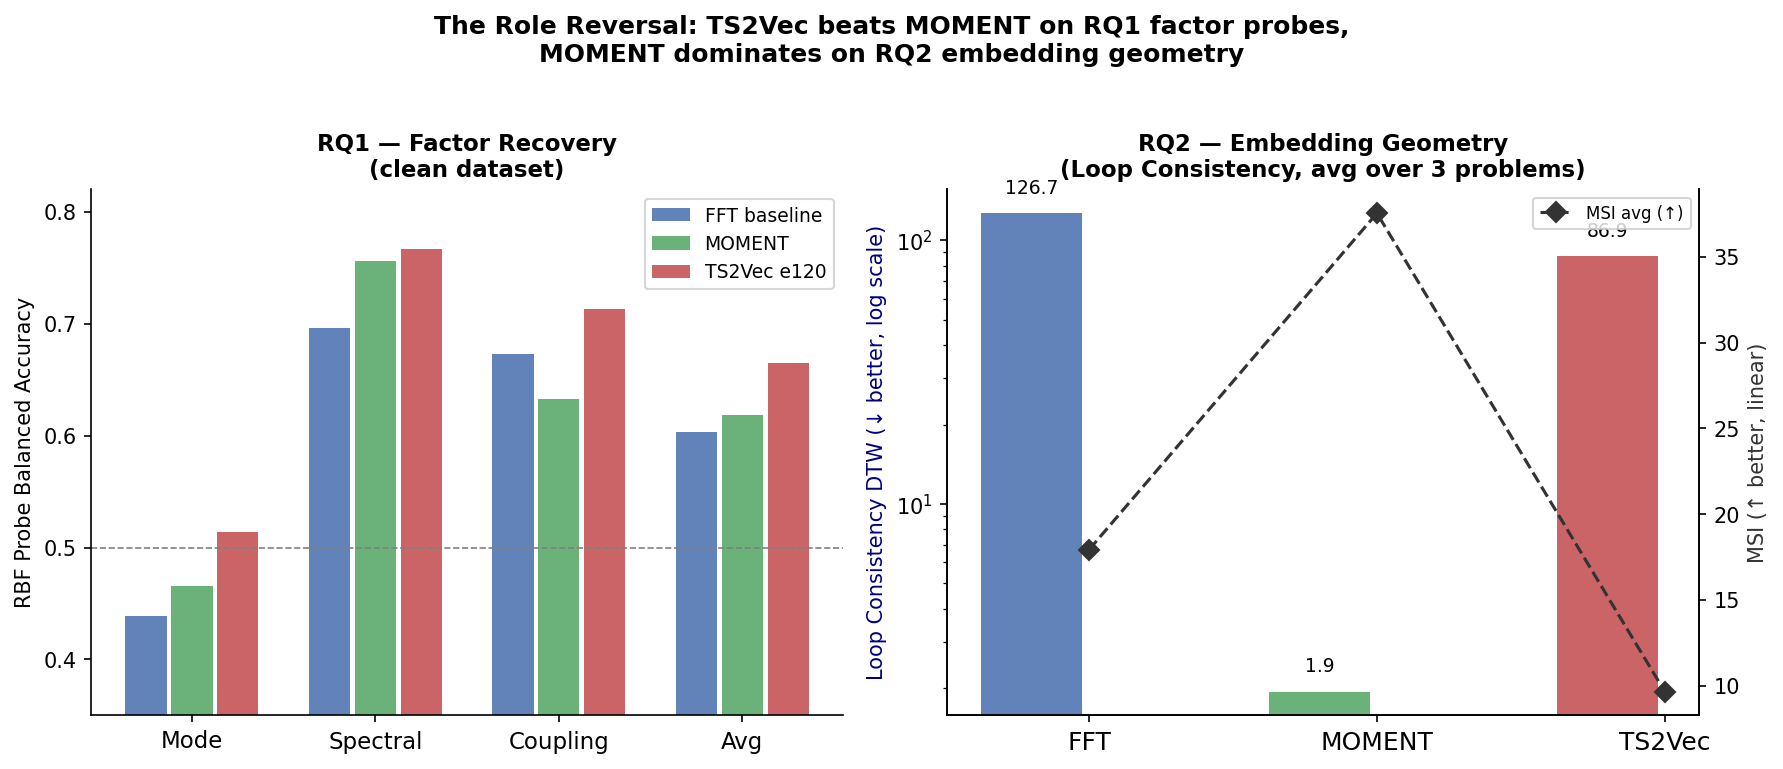
\includegraphics[width=\linewidth]{figures/fig7_role_reversal.png}
\caption{Role reversal}
\end{figure}

One of the most striking findings across all experiments is a \textbf{consistent role reversal} between
MOMENT and TS2Vec:

\begin{longtable}{|l|l|l|}
\hline
\textbf{} & \textbf{RQ1 (factor recovery probes)} & \textbf{RQ2 (embedding geometry)} \\
\hline
\endfirsthead
\hline
\textbf{} & \textbf{RQ1 (factor recovery probes)} & \textbf{RQ2 (embedding geometry)} \\
\hline
\endhead
\hline
\endfoot
MOMENT & 61.8\% avg balanced acc --- middle & Loop DTW \textasciitilde{}1.5 --- \textbf{dominant} \\
\hline
TS2Vec e120 & 66.5\% avg balanced acc --- \textbf{best} & Loop DTW \textasciitilde{}87 --- worst \\
\hline
\end{longtable}

TS2Vec's contrastive training pushes same-window representations together globally, which helps
linear/RBF probes recover discrete factor labels --- but the geometry is chaotic, loops don't form,
centroids drift. MOMENT's pretrained features produce geometrically regular embeddings --- tight,
stable, fast mode transitions --- without any task-specific training.

\textbf{These are complementary strengths.} TS2Vec for discrete label recovery; MOMENT for continuous
online monitoring and anomaly detection.

\subsubsection{13.2 MOMENT vs FFT: When Each Wins}

Across all five RQs, two conditions predict which model wins on MSI:

\begin{longtable}{|l|l|l|}
\hline
\textbf{Condition} & \textbf{MOMENT wins MSI} & \textbf{FFT wins MSI} \\
\hline
\endfirsthead
\hline
\textbf{Condition} & \textbf{MOMENT wins MSI} & \textbf{FFT wins MSI} \\
\hline
\endhead
\hline
\endfoot
Clean, periodic, sine signals & ✓ (RQ3 noise\_000: 73.1 vs 37.2) &  \\
\hline
High noise, periodic signals & ✓ (RQ3 noise\_040: 59.9 vs 22.8) &  \\
\hline
Chirp / damped / sawtooth signals & ✓ (RQ6: 51--57 vs 19--25) &  \\
\hline
Mixed step+sine channels (1--3 step ch) & ✓ (RQ6: 48--73 vs 17--28) &  \\
\hline
Pure step-change signals &  & ✓ (RQ3 sig\_step: 9.6 vs 2.8) \\
\hline
Event/impulse signals &  & ✓ (RQ3 sig\_event: 23.9 vs 18.7) \\
\hline
CNC machining, program steps &  & ✓ (RQ4: 45--82 vs 36--55) \\
\hline
CNC machining, operating states & \textasciitilde{}tied & \textasciitilde{}tied \\
\hline
Small window (ws=32) &  & ✓ FFT closer \\
\hline
Optimal window (ws=64) &  & ✓ FFT 64.3 vs MOMENT 48.6 \\
\hline
\end{longtable}

MOMENT wins whenever the signal is periodic and smooth. FFT wins (or ties) whenever the signal
has strong spectral structure that a simple amplitude spectrum captures completely, or when the
signal is non-periodic. On geometry metrics (loop DTW, centroid stability), MOMENT wins
\textbf{always and by a large margin} regardless of condition.

\subsubsection{13.3 The Loop Consistency Invariant}

Across all 5 RQs, MOMENT loop DTW is bounded between 1.25 and 11.1 regardless of noise level,
missing data type, number of modes, signal type, window size, or scenario complexity. FFT loop
DTW ranges from 66 (best case P1) to 2214 (cnc\_two\_parts op-state). This suggests MOMENT's
pretrained representation has a structural property that enforces temporal consistency in a
way FFT does not --- likely the transformer's attention mechanism averaging over the full window
context rather than computing a fixed spectral decomposition.

\subsubsection{13.4 Production Risk Summary}

\begin{longtable}{|l|l|l|}
\hline
\textbf{Risk} & \textbf{FFT} & \textbf{MOMENT} \\
\hline
\endfirsthead
\hline
\textbf{Risk} & \textbf{FFT} & \textbf{MOMENT} \\
\hline
\endhead
\hline
\endfoot
Sensor dropout (channel missing) & \textbf{Critical} --- MSI 13.5, loop DTW 478 & Not measured --- likely critical \\
\hline
High noise ($\sigma$ = 0.40) & Moderate --- MSI drops 38\% & Low --- MSI drops 18\% \\
\hline
Step/event signal type & Moderate --- MSI 9.6 & \textbf{Severe} --- MSI 2.8 \\
\hline
Many modes (K=8) & Moderate --- MSI 30.9 & Low --- MSI 52.2 \\
\hline
Small window (ws=32) & Moderate & Low (padding robust at ws=64+) \\
\hline
Large window (ws$\geq$256) & \textbf{Severe} --- MSI collapses & Moderate --- more stable \\
\hline
\end{longtable}

\vspace{4pt}\hrule\vspace{4pt}

\subsection{14. Lessons Learned}

\subsubsection{14.1 Method Design}

\begin{longtable}{|l|l|l|}
\hline
\textbf{\#} & \textbf{Lesson} & \textbf{Evidence} \\
\hline
\endfirsthead
\hline
\textbf{\#} & \textbf{Lesson} & \textbf{Evidence} \\
\hline
\endhead
\hline
\endfoot
L1 & Temporal-neighbour contrastive pairs teach temporal proximity, not mode identity. & Phase 1--2: baselines beat learned \\
\hline
L2 & Reconstruction loss adds complexity but doesn't fix misaligned objectives. & Phase 2 vs 1: no improvement \\
\hline
L3 & More training helps probes but can harm global structure. & TS2Vec e80$\rightarrow$e120: coupling ARI 0.006$\rightarrow$0.004 \\
\hline
L4 & Pretrained foundation models give strong geometry without task-specific training. & RQ1/RQ2 role reversal \\
\hline
L5 & Load (continuous amplitude) is not learnable from the current setup --- R$^2$$\leq$0 for all methods. & RQ1 Table 1 \\
\hline
L6 & MOMENT's pretraining assumption fails on \textit{purely} step/event signals --- but mixed signals still favour MOMENT. & RQ3 sig\_step MSI 2.8; RQ6 ratio\_4step MSI 27.7 vs 9.6 \\
\hline
L7 & Channel dropout is a critical production failure mode for all tested methods. & RQ3 miss\_channel: FFT MSI 13.5, loop DTW 478 \\
\hline
L8 & MOMENT loop consistency is an invariant: \textasciitilde{}0.002 centroid stability regardless of signal type, window size, or noise. & RQ6: all 8 scenarios show centroid stability 0.002 \\
\hline
L9 & Exotic continuous signals (chirp, damped, sawtooth) favour MOMENT strongly --- FFT MSI drops 49\% on chirp. & RQ6 sig\_chirp: FFT 18.9, MOMENT 54.8 \\
\hline
\end{longtable}

\subsubsection{14.2 Evaluation Design}

\begin{longtable}{|l|l|l|}
\hline
\textbf{\#} & \textbf{Lesson} & \textbf{Evidence} \\
\hline
\endfirsthead
\hline
\textbf{\#} & \textbf{Lesson} & \textbf{Evidence} \\
\hline
\endhead
\hline
\endfoot
L8 & Retrieval R@K is misleading when training biases nearest neighbours. & Phase 2: R@5 > 0.96 but probe accuracy 27\% \\
\hline
L9 & Single-seed results for TS2Vec should be treated cautiously. & MOMENT coupling std $\pm$0.042 \\
\hline
L10 & Geometry metrics reveal embedding quality that probe accuracy misses. & MOMENT dominates RQ2 while middle of pack in RQ1 \\
\hline
L11 & PCA compactness may penalise high-dimensional embeddings unfairly. & MOMENT PCA compact 1.63--7.97 vs FFT 0.26--0.33 \\
\hline
L12 & Window size must be smaller than the shortest mode segment duration. & RQ5: op-state MSI=0 at ws$\geq$256 \\
\hline
\end{longtable}

\subsubsection{14.3 Benchmark Design}

\begin{longtable}{|l|l|l|}
\hline
\textbf{\#} & \textbf{Lesson} & \textbf{Evidence} \\
\hline
\endfirsthead
\hline
\textbf{\#} & \textbf{Lesson} & \textbf{Evidence} \\
\hline
\endhead
\hline
\endfoot
L13 & FRS is a valid instrument for spectral/mode learning but doesn't capture step signals, discrete channels, or mixed signal types from real PLC logs. & RQ3 signal-type axis \\
\hline
L14 & High baseline performance (FFT avg 60.3\%) indicates strong spectral structure --- learned methods must beat it by a meaningful margin. & RQ1 Table 2: +6.2pp gap \\
\hline
L15 & Missing data stress-testing is essential before production recommendation. & RQ3: block-missing drops MOMENT MSI 44\% \\
\hline
L16 & Two-level label structure (coarse/fine) reveals that the same embedding cannot optimise both simultaneously. & RQ4: FFT wins on fine (program step), ties on coarse (op-state) \\
\hline
\end{longtable}

\vspace{4pt}\hrule\vspace{4pt}

\subsection{15. Open Questions}

\begin{enumerate}
  \item \textbf{Why does MOMENT fail so severely on step signals?} MSI 2.8 on sig\_step while retaining
\end{enumerate}
   loop DTW 10.4 --- the orbits are consistent but entirely overlapping. Is the T5 backbone
   averaging out the step transitions into a smooth mean?

\begin{enumerate}
  \item \textbf{Can factor-aware pairs fix the load problem?} Windows with matching load values as positives
\end{enumerate}
   instead of temporal neighbours --- the most direct fix for Load R$^2$$\leq$0.

\begin{enumerate}
  \item \textbf{Does MOMENT's loop consistency invariant hold under channel dropout?} The miss\_channel
\end{enumerate}
   scenario was not evaluated for MOMENT. If loop DTW is still low despite collapsed MSI,
   it has important implications for fault-tolerant monitoring architectures.

\begin{enumerate}
  \item \textbf{What is the optimal ensemble?} RQ4 shows FFT and MOMENT have complementary strengths:
\end{enumerate}
   FFT for MSI / label classification, MOMENT for loop consistency / anomaly detection.
   A simple ensemble (MOMENT geometry for anomaly detection + FFT features for mode
   classification) might outperform either alone.

\begin{enumerate}
  \item \textbf{Would DCC (contrastive training with factor-aware pairs) break the role reversal?}
\end{enumerate}
   The RQ3 DCC training jobs failed due to an import bug (now fixed). Running DCC would tell
   us whether a trained model can achieve both high probe accuracy (like TS2Vec) and
   good geometry (like MOMENT).

\begin{enumerate}
  \item **Why does MOMENT perform so much better in RQ6 ratio\_4step (MSI 27.7) than RQ3 sig\_step
\end{enumerate}
   (MSI 2.8) if both are pure step-channel?** The mode-level step amplitude patterns in RQ6
   likely differ across modes (each mode has a fixed level per channel), whereas RQ3 sig\_step
   used level differences that overlapped. Confirms that the signal-type failure is amplitude
   overlap, not just aperiodicity.

\begin{enumerate}
  \item \textbf{Does ws=64 generalise across scenarios?} RQ5 only tested one scenario (cnc\_part\_full).
\end{enumerate}
   The optimal window size likely varies with spindle speed --- at high RPM, 64 samples may
   capture less than one vibration cycle.

\vspace{4pt}\hrule\vspace{4pt}

\subsection{16. What Remains To Be Done}

\subsubsection{Immediate}

\begin{enumerate}
  \item \textbf{RQ3 DCC training} --- resubmit \texttt{rq3\_dcc.slurm} (import bug fixed). Will add a trained
\end{enumerate}
   contrastive baseline to the RQ3 landscape sweep.
\begin{enumerate}
  \item \textbf{Sync RQ3--5 results locally} --- rsync results and plots from Alvis.
  \item \textbf{RQ2 visualisation plots} --- the viz step failed for RQ2 eval due to missing matplotlib;
\end{enumerate}
   regenerate locally.

\subsubsection{Track A --- FRS Fixes (highest priority)}

\begin{itemize}
  \item \textbf{A1}: Factor-aware positive pairs for TS2Vec (fix load and coupling learning)
  \item \textbf{A2}: Load regression auxiliary head
  \item \textbf{A4}: Multi-seed TS2Vec to quantify variance
  \item \textbf{A3}: OOD splits (unseen factor combinations at test time)
  \item \textbf{A5}: Segment-level change-point detection evaluation
\end{itemize}

\subsubsection{Track B --- PLC Log Bridge}

\begin{itemize}
  \item \textbf{B1}: Synthetic PLC log corpus with FRS-like factors and mixed signal types
  \item \textbf{B2}: Tabular/numerical embedding extraction with step-aware encoding
  \item \textbf{B3}: Cross-modal comparison with FRS eval infrastructure
\end{itemize}

\subsubsection{Track C --- Geometry and Architecture}

\begin{itemize}
  \item Replace PCA compactness with silhouette score in the full embedding space
  \item Test MOMENT with fine-tuning on a small labelled set (few-shot regime)
  \item Investigate whether a lightweight adapter on MOMENT's 768-dim output can recover
\end{itemize}
  the Load factor that frozen MOMENT misses

\end{document}